\documentclass[14pt]{extreport}
\usepackage{gost}
\usepackage{tikz}
\usepackage{listings}
\usetikzlibrary{shapes.geometric}
\begin{document}
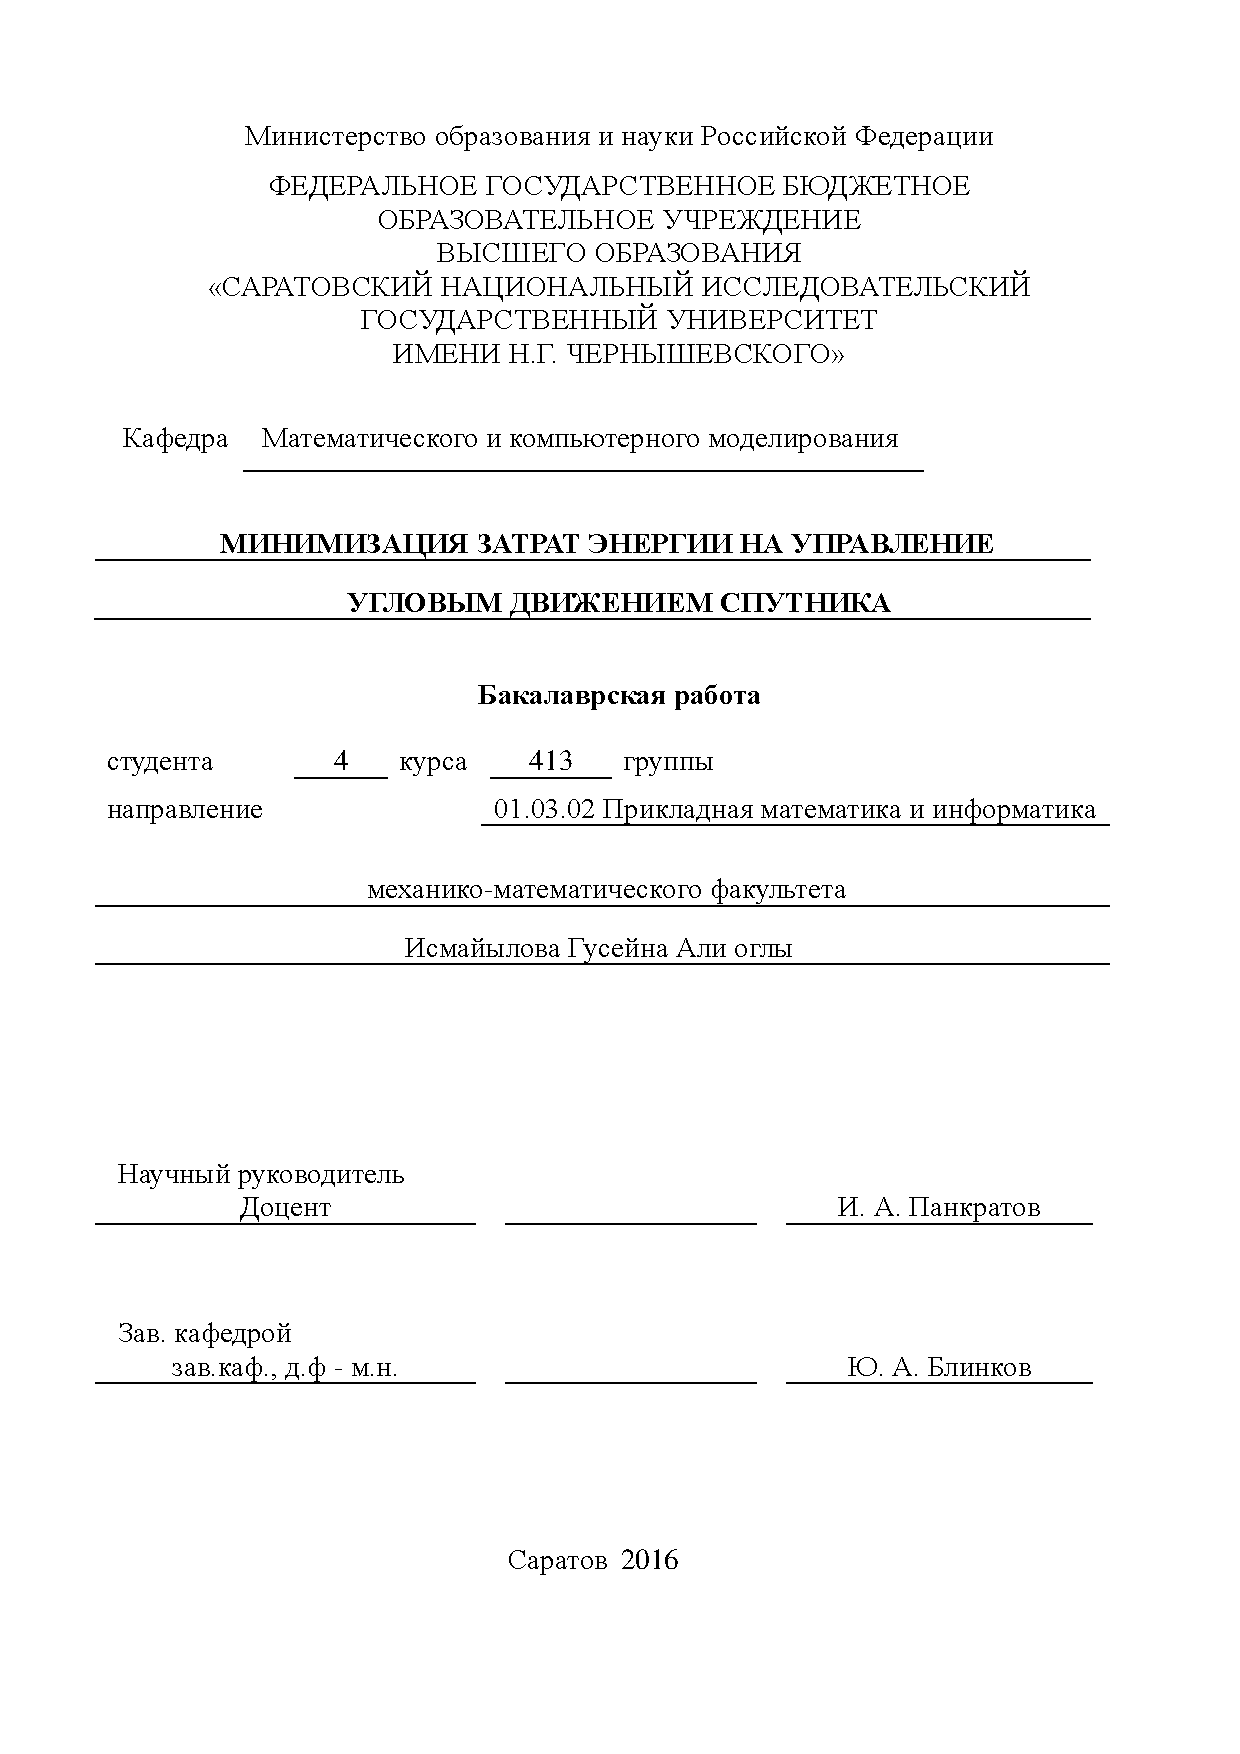
\includepdf[pages={1}]{titulDiplom.pdf}

\tableofcontents


\abbrevdef


$\mathbb{R}_3$ --- трёхмерное вещественное векторное пространство с введённым на нём положительно определённым скалярным произведением.

Норма --- функционал, заданный на векторном пространстве и обобщающий понятие длины вектора или абсолютного значения числа.

ИСЗ --- искусственный спутник Земли.

Кинематика --- раздел механики, изучающий математическое описание (средствами геометрии, алгебры, математического анализа)
движения идеализированных тел (материальная точка, абсолютно твердое тело, идеальная жидкость),
без рассмотрения причин движения (массы, сил и т. д.).

Базис --- множество таких векторов в векторном пространстве, что любой вектор этого пространства может быть единственным
образом представлен в виде линейной комбинации векторов из этого множества — базисных векторов.

Инерциальная система отсчёта (ИСО) — система отсчёта, в которой все свободные тела движутся прямолинейно и равномерно, либо покоятся. 



\intro

Выполненная квалификационная работа посвящена задаче оптимального управления углового движения искусственного спутника Земли (ИСЗ), 
для которой требуется составить и решить краевую задачу с помошью принципа максимума Л.С. Понтрягина.
Управление --- вектор угловой скорости ИСЗ. Необходимо рассмотреть случай минимизации энергии на перевод ИСЗ в нужное угловое положение.
Время окончания процесса фиксировано. Также требуется рассмотреть задачу с её различными параметрами и вывести основные закономерности.

Теория управления является в настоящее время быстро развивающимся разделом современной математики, что
вызвано потребностями многочисленных приложений в таких разнообразных
дисциплинах как аэрокосмические науки, инженерные и технические науки, гибридные
системы, вычислительные и
компьютерные науки, океанографические, физические и математические науки. Возрастает интерес к теории оптимального управления
и ее приложениям у математиков, экономистов и специалистов по проблемам окружающей среды, а также международных научных организаций, что
подтверждается увеличением количества работ в российских и зарубежных издательствах.

Основополагающее значение в теории оптимального управления имеет принцип максимума Л.С. Понтрягина,
который получил развитие и приложение в работах российских и зарубежных математиков.

Научая новизна данной работы состоит в рассмотрении поставленной задачи с применением алгебры кватернионов не только в теоретических выкладках,
но и в программной реализации решения, которая является универсальной для любого типа задач управления благодаря использованию интерфейсов
в программе, которые могут быть ипользованы для самых различных уравнений состояния [19].

В данной работе будут представлены основные определения, понятния и теоремы, которые позволят составить и решить поставленную задачу,
решение которой состоит из двух частей: аналитической и численной. Аналитическая часть позволяет перевести задачу оптимального управления
к краевой задаче, для которой составлен алгоритм в численной части. Для реализации такого алгоритма была написана программа,
которая выдает результаты решения краевой задачи, а также генерирует скрипт для графиков, которые наглядным образом отражают
суть этих результатов.


\chapter{Алгебра кватернионов}

Будем рассматривать кватернион как математический объект $\boldsymbol{\Lambda}(\lambda_0,\ \overline{\lambda})$,
где $\lambda_0$ --- скалярная величина, $\overline{\lambda}$ --- вектор в $\mathbb{R}_3$.
Кватернион также можно представить в виде четырехмерного гиперкомплексного числа:

\begin{equation}
 \boldsymbol\Lambda = \lambda_0\ + \ i_1\lambda_1\ + \ i_2\lambda_2\ + \ i_3\lambda_3,
\end{equation}
где $\lambda_k,\ k\ =\ \overline{0, 3}$ --- действительные числа, $i_1,\ i_2,\ i_3$ --- кватернионные единицы, обладающие свойством: 
$i_1^2\ =\ i_2^2\ =\ i_3^2\ =\ i_1i_2i_3\ =\ -1.$

Операции с кватернионами:
\begin{itemize}
\item[1)] $\boldsymbol{\Lambda_1}(\lambda_{01},\ \overline{\lambda_1})\ \pm\ \boldsymbol{\Lambda_2}(\lambda_{02},\ \overline{\lambda_2}) =
\boldsymbol\Lambda(\lambda_{01}\ \pm\ \lambda_{02},\ \overline{\lambda_1}\ \pm\ \overline{\lambda_2}),$
\item[2)] $\alpha\boldsymbol\Lambda(\lambda_{0},\ \overline{\lambda})\ =\ \boldsymbol\Lambda(\alpha\lambda_{0},\ \alpha\overline{\lambda}),\ \alpha - const,$ 
\item[3)] $\boldsymbol{\Lambda_1}(\lambda_{01},\ \overline{\lambda_1})\ \circ\ \boldsymbol{\Lambda_2}(\lambda_{02},\ 
\overline{\lambda_2})\ =\ \boldsymbol\Lambda(\lambda_{01}\lambda_{02}\ -\ (\overline{\lambda_1},\ \overline{\lambda_2}),
\lambda_{01}\overline{\lambda_2}\ +\ \lambda_{02}\overline{\lambda_{1}}\ +\ \overline{\lambda_{1}}\ \times\ \overline{\lambda_{2}})$
(умножение кватернионов),
\item[4)] $||\boldsymbol\Lambda(\lambda_{0},\ \overline{\lambda})||\ =\ \sqrt{\lambda_{0}^2\ +\ (\overline{\lambda},\ \overline{\lambda})}$ (норма кватерниона),
\item[5)] $\widetilde{\boldsymbol\Lambda}\ =\ \boldsymbol\Lambda(\lambda_{0},\ -\overline{\lambda})$ (сопряженный кватернион к $\boldsymbol\Lambda(\lambda_{0},\ \overline{\lambda})$),
\item[6)] $\boldsymbol\Lambda^{-1}\ =\ \dfrac{\widetilde{\boldsymbol\Lambda}}{||\boldsymbol\Lambda||^2} $ (обратный кватернион к $\boldsymbol\Lambda(\lambda_{0},\ \overline{\lambda})$).
\end{itemize}

Свойства операций с кватернионами:

\begin{itemize}
\item[1)] $\boldsymbol\Lambda\ \circ\ (\boldsymbol{M}\ \circ\ \boldsymbol{N})\ =\ (\boldsymbol\Lambda\ \circ\ \boldsymbol{M})\ \circ\ \boldsymbol{N}$,
\item[2)] $\boldsymbol\Lambda\ \circ\ (\boldsymbol{M}\ +\ \boldsymbol{N})\ =\ \boldsymbol\Lambda\ \circ\ \boldsymbol{M}\ +\ \boldsymbol\Lambda\ \circ\ \boldsymbol{N}$,
\item[3)] $\boldsymbol{\Lambda_1}\ \circ\ \boldsymbol{\Lambda_2}\ \neq\ \boldsymbol{\Lambda_2}\ \circ\ \boldsymbol{\Lambda_1}$.
\end{itemize}

Кватернионы используются для описания поворота твердого тела [1][2]. Именно с помошью алгебры кватернионов
будет поставлена задача в работе, это позволит упростить вычисления и программную реализацию её решения. 

\newpage

\chapter{Кинематика вращения твердого тела}

Рассмотрим следующие теоремы и утверждения, которые позволят корректно поставить и решить задачу в данной работе [6].

\textbf{Теорема 1.} (\textit{о положении твердого тела}). Произвольное положение твердого тела с
неподвижной точкой задается нормированным кватернионом $\Lambda$ по формулам

\begin{equation}
 \overline{e_k}\ =\ \boldsymbol\Lambda\ \circ\ \overline{i_{k}}\ \circ\ \boldsymbol{\widetilde{\Lambda}},\ k = \overline{1,\ 3},
\end{equation}
где базис $e_k$ связан с самим телом, а базис $i_k$ является неподвижным.
\newline

\textbf{Теорема 2.} (\textit{о повороте базиса}). Единичный кватернион вида $\Lambda(\textrm{cos}(\varphi/2)),\ \overline{e} \textrm{sin}(\varphi/2))$
задает поворот вокруг единичного вектора $\overline{e}$ на угол $\varphi$.
\newline

\textbf{Теорема 3.} (\textit{о конечном повороте}). Любое положение твердого тела с неподвижной точкой может быть получено
одним поворотом вокруг оси $\overline{e}\ =\ \dfrac{\overline{\lambda}}{|\overline{\lambda}|}$ на угол $\varphi\ =\ \textrm{2arccos}\lambda_0$,
где $\boldsymbol\Lambda(\lambda_0,\ \overline{\lambda})$ --- нормированный кватернион, задающий положение тела.
\newline

\textbf{Теорема 4.} (\textit{о сложении поворотов}). Пусть кватернион $\boldsymbol{\Lambda_1}$ задает поворот из базиса $i^{(1)}_k$
в базис $i^{(2)}_k,\ k = \overline{1,\ 3}$, а кватенион $\boldsymbol{\Lambda_2}$ --- поворот из базиса $i^{(2)}_k$ в $i^{(3)}_k$.
Тогда кватернион результирующего поворота $\boldsymbol\Lambda$ будет равен $\boldsymbol\Lambda\ =\ \boldsymbol{\Lambda_1}\ \circ\ \boldsymbol{\Lambda_2}$.
\newline

\textbf{Следствие из теоремы 4.} Для того, чтобы выполнить $n$ последовательных поворотов из базиса $i^{(1)}_k$ 
в базис $i^{(n)}_k,\ k\ =\ \overline{1, 3}$, необходимо найти кватернион $\Lambda$, который задается следующей формулой

\begin{equation}
 \boldsymbol\Lambda\ =\ \boldsymbol{\Lambda_1}\ \circ\ \boldsymbol{\Lambda_2}\ \circ\ ...\ \circ\ \boldsymbol{\Lambda_n},
\end{equation}
где $\boldsymbol{\Lambda_k},\ k = \overline{1,\ n}$ задает поворот из базиса $I^{(k-1)}$ в базис $I^{(k)}$. 
\newline

Так как поворот абсолютно твердого тела в трёхмерном евклидовом пространстве задается углами Эйлера [14]: $\alpha,\ \beta,\ \gamma$ (рис. 2.1),
то для определения кватерниона, который выражает эти углы, необходимо воспользоватся формулой $(2.2)$, которая в данном случае принимает вид

\begin{equation}
 \boldsymbol\Lambda\ =\ \boldsymbol{\Lambda_1}\ \circ\ \boldsymbol{\Lambda_2}\ \circ\ \boldsymbol{\Lambda_3},
\end{equation}
где по \textbf{теореме 2} $\boldsymbol{\Lambda_1},\ \boldsymbol{\Lambda_2},\ \boldsymbol{\Lambda_3}$ определяются следующими соотношениями

\begin{equation}
\begin{cases}
 \boldsymbol\Lambda_1\ =\ \boldsymbol{\Lambda_1}\big(cos (\alpha/2),\ (0,\ 0,\ sin(\alpha/2))\big), \\ 
 \boldsymbol\Lambda_2\ =\ \boldsymbol{\Lambda_2}\big(cos (\beta/2),\ (0,\ sin(\beta/2),\ 0)\big), \\ 
 \boldsymbol\Lambda_3\ =\ \boldsymbol{\Lambda_3}\big(cos (\gamma/2),\ (sin(\gamma/2),\ 0,\ 0)\big). \\ 
\end{cases}
\end{equation}

\begin{center}
 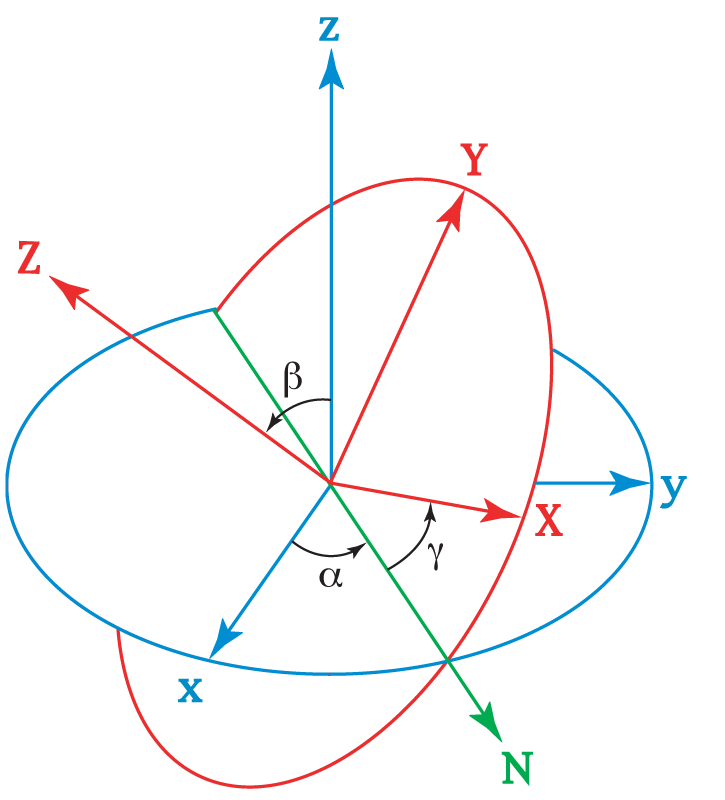
\includegraphics[width=8cm, height=8cm]{1.png}
 
 Рисунок 2.1 --- углы Эйлера
\end{center}

Из $(3.3)$ получаем связь компонент кватерниона и углов Эйлера [15]

\begin{equation}
\begin{cases}
 \boldsymbol{\Lambda}\ =\ \boldsymbol\Lambda(\lambda_0,\ \lambda_1,\ \lambda_2,\ \lambda_3), \\
 \lambda_0\ =\ cos(\gamma/2) cos(\beta/2) cos(\alpha/2)\ +\ sin(\gamma/2) sin(\beta/2) sin(\alpha/2), \\
 \lambda_1\ =\ sin(\gamma/2) cos(\beta/2) cos(\alpha/2)\ -\ cos(\gamma/2) sin(\beta/2) sin(\alpha/2), \\
 \lambda_2\ =\ cos(\gamma/2) sin(\beta/2) cos(\alpha/2)\ +\ sin(\gamma/2) cos(\beta/2) sin(\alpha/2), \\
 \lambda_3\ =\ cos(\gamma/2) cos(\beta/2) sin(\alpha/2)\ -\ sin(\gamma/2) sin(\beta/2) cos(\alpha/2). 
 \end{cases}
\end{equation}

Обратная связь выглядит следующим образом [15]

\begin{equation}
\begin{cases}
\gamma\ =\ arctg \ \dfrac{2(\lambda_0\lambda_1\ +\ \lambda_2\lambda_3)}{1\ -\ 2(\lambda_1^2\ +\ \lambda_2^2)}, \\ \\
\beta\ =\ arcsin (2(\lambda_0\lambda_2\ -\ \lambda_3\lambda_1)), \\ \\
\alpha\ =\ arctg \ \dfrac{2(\lambda_0\lambda_3\ +\ \lambda_1\lambda_2)}{1\ -\ 2(\lambda_2^2\ +\ \lambda_3^2)}.
 \end{cases}
\end{equation}

Пусть базис $i_k,\ k\ =\ \overline{1,\ 3}$ --- неподвижный, относительно которого движется тело с неподвижной точкой $O$,
и для любого момента $t$ задан базис $e_k(t),\ k\ =\ \overline{1,\ 3}$, который связан с телом. Тогда для некоторого промежутка времени $\Delta t$
тело можно повернуть на некоторый угол $\Delta\varphi(t,\ \Delta t)$, который переведет тело из одного базиса, связанный с телом,
в другой при начальном моменте времени $t$. При этом относительно неподвижного базиса тело будет двигаться
с некоторой угловой скоростью $\overline{\omega}$, которая задается следующим образом [7] 

\begin{equation}
  \overline{\omega}\ =\ \lim_{\Delta t\to 0} \dfrac{\Delta\varphi(t,\ \Delta t)}{\Delta t} \ \overline{e}(t,\ \Delta t).
\end{equation}

Перемещение из положениия $e_k(t)$ в положение $e_k(t\ +\ \Delta t)$ задается кватернионом

\begin{equation}
\delta\boldsymbol\Lambda\ =\ cos\ \dfrac{\Delta\varphi(t,\ \Delta t)}{2}\ +\ \overline{e}(t,\ \Delta t)\ sin\ \dfrac{\Delta\varphi(t,\ \Delta t)}{2}.
\end{equation}

Разложим функцию $cos\ \dfrac{\Delta\varphi(t,\ \Delta t)}{2}$ в ряд Тейлора до второго порядка точности, тогда $(2.8)$ примет вид

\begin{equation}
\delta\boldsymbol\Lambda\ =\ 1\ +\ \overline{e}(t,\ \Delta t)\ sin\ \dfrac{\Delta\varphi(t,\ \Delta t)}{2}\ +\ O((\Delta\varphi)^2).
\end{equation}

Так как $\boldsymbol\Lambda(t\ +\ \Delta t)\ =\ \delta\boldsymbol\Lambda\ \circ\ \Lambda(t)$,
то $\boldsymbol\Lambda(t\ +\ \Delta t)\ -\ \boldsymbol\Lambda(t)\ =\ \delta\boldsymbol\Lambda(t)\ -\ \boldsymbol\Lambda(t)\ \Rightarrow\ \Delta\boldsymbol\Lambda\
=\ (\delta\boldsymbol\Lambda\ -\ 1)\ \circ\ \boldsymbol\Lambda(t)$.

Из $(2.9)$ производная от $\boldsymbol\Lambda$ будет определяться следующим образом

\begin{multline*}
\boldsymbol{\dot{\Lambda}}\ =\ \lim_{\Delta t \to 0}\ \dfrac{\Delta\boldsymbol\Lambda}{\Delta t}\ =\ 
\lim_{\Delta t \to 0}\ \dfrac{\delta\boldsymbol\Lambda\ -\ 1}{\Delta t}\ \circ\ \boldsymbol\Lambda(t)\ =\
\lim_{\Delta t \to 0}\ \dfrac{\overline{e}(t,\ \Delta t)sin\ \dfrac{\Delta \varphi(t,\ \Delta t)}{2}}{\Delta t}\   \\ \\ \circ\ \boldsymbol\Lambda(t)\ = 
\lim_{\Delta t \to 0} \dfrac{\overline{e}(t,\ \Delta t)
\dfrac{\Delta \varphi(t,\ \Delta t)}{2}sin\dfrac{\Delta \varphi(t,\ \Delta t)}{2}}{\dfrac{\Delta \varphi(t,\ \Delta t)}{2} \Delta t}\ \circ\ \boldsymbol\Lambda(t) =   \\ \\
\lim_{\Delta t \to 0} \dfrac{\overline{e}(t,\ \Delta t)\Delta\varphi(t,\ \Delta t)}{2\Delta t}\ \cdot
\lim_{\Delta t \to 0}\dfrac{sin\dfrac{\Delta \varphi(t,\ \Delta t)}{2}}{\dfrac{\Delta \varphi(t,\ \Delta t)}{2}}\ \circ\ \boldsymbol\Lambda(t) =  \\ \\
\dfrac{1}{2}\lim_{\Delta t \to 0}\dfrac{\overline{e}(t,\ \Delta t)\Delta\varphi(t,\ \Delta t)}{\Delta t}\ \circ\ \boldsymbol\Lambda(t) = 
\dfrac{1}{2}\ \overline{\omega}\ \circ\ \boldsymbol\Lambda(t). 
\end{multline*}

Таким образом, связь между кватернионом $\Lambda$ и угловой скоростью $\overline{\omega}$ задается формулами

\begin{equation}
\boldsymbol{\dot{\Lambda}} = \dfrac{1}{2}\ \overline{\omega} \circ \boldsymbol\Lambda(t),
\end{equation}
\begin{equation}
\overline{\omega} = 2\boldsymbol{\dot{\Lambda}} \circ \boldsymbol{\widetilde{\Lambda}}.
\end{equation}

Полученные уравнения $(2.10), (2.11)$ называются уравнениями Пуассона [3][7]. Для удобства выполнения математических операций
в этих уравнениях угловую скорость $\overline{\omega}$ можно рассматривать как кватернион, скалярная часть которого равна нулю. 

\newpage

\chapter{Общая задача оптимального управления}

Определим задачу оптимального управления в общем случае, которая позволит в дальнейшем корректно сделать постановку задачи, рассматриваемой в данной работе.

Пусть положение тела описывается обыкновенным дифференциальным уравнением [3][4][11]

\begin{equation}
 \boldsymbol{\dot{\Lambda}}\ =\ F(t,\ \boldsymbol{\Lambda}(t),\ \boldsymbol\Omega(t)), 
\end{equation}
где $\boldsymbol\Lambda$ --- вектор состояния системы, $\boldsymbol\Omega$ --- вектор управления, $t$ --- время, $t\ \in T\ =\ [t_0,\ t_1]$ --- промежуток времени
функционирования системы.

$F(t,\ \boldsymbol\Lambda,\ \boldsymbol\Omega)$ --- непрерывная вместе со своими частными производными вектор -- функция. Также даны граничные условия

\begin{equation}
\begin{cases}
\boldsymbol\Lambda(t_0)\ =\ \boldsymbol{\Lambda_0}, \\
\boldsymbol\Lambda(t_1)\ =\ \boldsymbol{\Lambda_1}.
 \end{cases}
\end{equation}

Пусть качество управления системы определяется следующим функционалом [11]

\begin{equation}
I\ =\ \int_{t_0}^{t_1}F^0(t,\ \boldsymbol\Lambda(t),\ \boldsymbol\Omega(t))dt\ +\ F(t_1,\ \boldsymbol\Lambda(t_1)),
\end{equation}
где $F^0(t,\ \boldsymbol\Lambda,\ \boldsymbol\Omega)dt,\ F(t_1,\ \boldsymbol\Lambda)$ --- заданные непрерывно дифференцируемые функции, $t_1$ --- фиксировано.

Требуется найти такие $\boldsymbol\Lambda^*(t),\ \boldsymbol\Omega^*(t)$, чтобы функционал качества достигал своего минимума.
Искомые функции $\boldsymbol\Lambda^*(t),\ \boldsymbol\Omega^*(t)$ называются соответственно оптимальной траекторией и оптимальным управлением.

\textbf{Утверждение. }[11] Пусть существуют такие $\boldsymbol\Lambda^*(t),\ \boldsymbol\Omega^*(t)$, при которых функционал качества достигает своегоминимального значения,
тогда найдется такая вектор --- функция $\boldsymbol\Psi(t)\ =\ \boldsymbol\Psi(\boldsymbol{\Psi_1},\ \boldsymbol{\Psi_2},\ ...\ ,\ \boldsymbol{\Psi_n)}$, что:

\begin{itemize}
\item[1)] в каждой точке непрерывности управления $\boldsymbol\Omega^*(t)$ функция $H(t,\ \boldsymbol\Psi,\ \boldsymbol\Lambda^*,\ \boldsymbol\Omega)$ достигает максимума по управлению, то есть

\begin{equation}
 \max_{\boldsymbol\Omega \in D(\boldsymbol\Omega)} H(t,\ \boldsymbol\Psi(t),\ \boldsymbol\Lambda^*(t),\ \boldsymbol\Omega)\
 =\ H(t,\ \boldsymbol\Psi(t),\ \boldsymbol\Lambda^*(t),\ \boldsymbol\Omega^*(t)),
\end{equation}
где $D(\boldsymbol\Omega)$ --- область определения $\boldsymbol\Omega$, а $H(t,\ \boldsymbol\Psi,\ \boldsymbol\Lambda,\ \boldsymbol\Omega):$

\begin{equation}
 H(t,\ \boldsymbol\Psi,\ \boldsymbol\Lambda,\ \boldsymbol\Omega)\ =\ \sum_{j=1}^n\boldsymbol{\Psi_{j}}F_{j}(t,\ \boldsymbol\Lambda,\ \boldsymbol\Omega)\ -\ F^0(t,\ \boldsymbol\Lambda,\ \boldsymbol\Omega).
\end{equation}

\item[2)] функции $\boldsymbol\Omega^*(t),\ \boldsymbol\Psi(t)$ удовлетворяют системе уравнений

\begin{equation}
\begin{cases}
\boldsymbol{\dot{\Lambda}^{*}_j}(t)\ =\ \dfrac{\partial H(t,\ \boldsymbol\Psi(t),\ \boldsymbol{\Lambda^*}(t),\
\boldsymbol{\Omega^*}(t))}{ \partial \boldsymbol{\Psi_j}},\ \\ \\
\boldsymbol{\dot{\Lambda}^{*}_j}(t)\ =\ F_j(t,\ \boldsymbol{\Lambda^*}(t),\ \boldsymbol{\Omega^*}(t)),\\ \\
\boldsymbol{\Lambda_j^*}(t_0)\ =\ \boldsymbol{\Lambda_{0_j}},\\ \\
\boldsymbol{\dot{\Psi}_j}(t)\ =\ -\dfrac{\partial H(t,\ \boldsymbol\Psi(t),\ \boldsymbol\Lambda^*(t),\ \boldsymbol{\Omega^*}(t))}
{\partial \boldsymbol{\Lambda_j}},\ j\ =\ \overline{1,\ n}.
 \end{cases}
\end{equation}

\end{itemize}

Используемые в формулировке утверждения функции $\boldsymbol{\Psi_1},\ ...\ ,\ \boldsymbol{\Psi_n}$ называются вспомогательными переменными,
$H(t,\ \boldsymbol\Psi,\ \boldsymbol\Lambda,\ \boldsymbol\Omega)$ --- гамильтонианом, а $(3.6)$ --- системой канонических уравнений [11].

\newpage

\chapter{Постановка задачи для углового движения тела}
Пусть угловое движение тела описывается кинематическим уравнением Пуассона

\begin{equation}
2\dot{\boldsymbol\Lambda}\ =\ \boldsymbol\Lambda \circ \boldsymbol\Omega,
\end{equation}
где $\boldsymbol\Lambda\ =\ \boldsymbol\Lambda(\lambda_0,\ (\lambda_1,\ \lambda_2,\ \lambda_3))$ --- кватернион, характеризующий положение твердого тела относительно инерциальной системы координат,
$\boldsymbol\Omega\ =\ \boldsymbol\Omega(\omega_0,\ (\omega_1,\ \omega_2,\ \omega_3))$ --- кватернион, векторная часть которого равна абсолютной угловой скорости твердого тела относительно этой системы,
а скалярная часть равна нулю.

Выражение $(4.1)$ в развернутом виде выглядит следующим образом

\begin{equation}
\begin{cases}
2\dot{\lambda_0}\ =\ -\lambda_1\omega_1\ -\ \lambda_2\omega_2\ -\ \lambda_3\omega_3, \\
2\dot{\lambda_1}\ =\ \lambda_0\omega_1\ +\ \lambda_2\omega_3\ -\ \lambda_3\omega_2, \\
2\dot{\lambda_2}\ =\ \lambda_0\omega_2\ +\ \lambda_3\omega_1\ -\ \lambda_1\omega_3, \\
2\dot{\lambda_3}\ =\ \lambda_0\omega_3\ +\ \lambda_1\omega_2\ -\ \lambda_2\omega_1.
 \end{cases}
\end{equation}

Также дано начальное угловое положение 

\begin{equation}
\boldsymbol\Lambda(0)\ =\ \boldsymbol{\Lambda^0}.
\end{equation}
И конечное угловое положение

\begin{equation}
\boldsymbol\Lambda(T)\ =\ \boldsymbol{\Lambda^T}.
\end{equation}

Требуется найти такое оптимальное управление $\boldsymbol\Omega(t)$, чтобы функционал качества 

\begin{equation}
I\ =\ \int\limits_{0}^{T}(\alpha_1\omega_1\ +\ \alpha_2\omega_2\ +\ \alpha_3\omega_3)dt
\end{equation}
принимал минимальные значения при фиксированном $T$,
где $\alpha_1,\ \alpha_2,\ \alpha_3\ =\ \textrm{const}\ >\ 0$ --- весовые множители функционала $(4.5)$, $\omega_1,\ \omega_2,\ \omega_3$ 
--- компоненты векторной части $\Omega$.

Функционал качества $(4.5)$ характеризует общие энергетические затраты на управление.
Для начала задача будет решена в общем случае, а затем будут рассмотрены конкретные примеры.

\newpage

\chapter{Решение задачи с помощью принципа максимума Понтрягина}


Воспользуемся методом максимума Понтрягина, суть которого заключается в том, что задача оптимального управления сводится к решению краевой задачи
для системы обыкновенных дифференциальных уравнений. Для этого составляется функция Гамильтона -- Понтрягина: [3][4]

\begin{equation}
H\ =\ - f_0(\boldsymbol\Lambda,\ \boldsymbol\Omega,\ t)\ +\ \sum_{i\ =\ 1}^{3}\psi_i f_i(\boldsymbol\Lambda,\ \boldsymbol\Omega,\ t),
\end{equation}
где $\boldsymbol\Lambda\ =\ \boldsymbol\Lambda(\lambda_0,\ (\lambda_1,\ \lambda_2,\ \lambda_3))$,
$\boldsymbol\Omega\ =\ \boldsymbol\Omega(\omega_0,\ (\omega_1,\ \omega_2,\ \omega_3))$,
$\psi_i,\ i\ =\ \overline{0,3}$ --- вспомогательные сопряженные переменные, которые удовлетворяют следующим условиям

\begin{equation}
\dfrac{d\psi_i}{dt}\ =\ -\dfrac{\partial H}{\partial \lambda_i}.
\end{equation}
$f_0$ представляет собой подинтегральное выражения функционала качества $(4.5)$:

\begin{equation}
f_0\ =\ \alpha_1\omega_1\ +\ \alpha_2\omega_2\ +\ \alpha_3\omega_3.
\end{equation}
$f_i$ --- это компоненты кватерниона $\dfrac{1}{2}\boldsymbol\Lambda\ \circ\ \boldsymbol\Omega$, то есть

\begin{equation}
\begin{cases}
f_0\ =\ -\dfrac{1}{2}(\lambda_1\omega_1\ +\ \lambda_2\omega_2\ +\ \lambda_3\omega_3), \\ \\
f_1\ =\ -\dfrac{1}{2}(\lambda_0\omega_1\ +\ \lambda_2\omega_3\ -\ \lambda_3\omega_2), \\ \\ 
f_2\ =\ -\dfrac{1}{2}(\lambda_0\omega_2\ +\ \lambda_3\omega_1\ -\ \lambda_1\omega_3), \\ \\
f_3\ =\ -\dfrac{1}{2}(\lambda_0\omega_3\ +\ \lambda_1\omega_2\ -\ \lambda_2\omega_1). 
 \end{cases}
\end{equation}
\newline

Таким образом функция $H$ принимает вид

\begin{multline}
H = \alpha_1\omega_1 + \alpha_2\omega_2 + \alpha_3\omega_3 - 
\dfrac{1}{2}\psi_0(\lambda_1\omega_1 + \lambda_2\omega_2 + \lambda_3\omega_3) - 
\dfrac{1}{2}\psi_1(\lambda_0\omega_1 + \lambda_2\omega_3 - \lambda_3\omega_2) - \\
\dfrac{1}{2}\psi_2(\lambda_0\omega_2 + \lambda_3\omega_1 - \lambda_1\omega_3) - 
\dfrac{1}{2}\psi_3(\lambda_0\omega_3 + \lambda_1\omega_2 - \lambda_2\omega_1).
\end{multline}

Распишем условия $(5.2)$, для этого найдем частные производные $\dfrac{\partial H}{\partial \lambda_i}, i = \overline{0,\ 3}$:

\begin{equation}
\begin{cases}
 \dfrac{\partial H}{\partial \lambda_0}\ =\ \dfrac{1}{2}\big(\psi_1\omega_1\ +\ \psi_2\omega_2\ +\ \psi_3\omega_3 \big), \\ \\
 \dfrac{\partial H}{\partial \lambda_1}\ =\ \dfrac{1}{2}\big(- \psi_0\omega_1\ -\ \psi_2\omega_3\ +\ \psi_3\omega_2 \big), \\ \\
 \dfrac{\partial H}{\partial \lambda_2}\ =\ \dfrac{1}{2}\big(- \psi_0\omega_2\ -\ \psi_3\omega_1\ +\ \psi_1\omega_3 \big), \\ \\
 \dfrac{\partial H}{\partial \lambda_3}\ =\ \dfrac{1}{2}\big(- \psi_0\omega_3\ -\ \psi_1\omega_2\ +\ \psi_2\omega_1 \big). 
 \end{cases}
\end{equation}

Таким образом, уравнения для параметров $\psi_i,\ i\ =\ \overline{0,\ 3}$ выглядят следующим способом

\begin{equation}
\begin{cases}
 2\dot{\psi_0}\ =\ - \psi_1\omega_1\ -\ \psi_2\omega_2\ -\ \psi_3\omega_3, \\
 2\dot{\psi_1}\ =\ \psi_0\omega_1\ +\ \psi_2\omega_3\ -\ \psi_3\omega_2, \\
 2\dot{\psi_2}\ =\ \psi_0\omega_2\ +\ \psi_3\omega_1\ -\ \psi_1\omega_3, \\
 2\dot{\psi_3}\ =\ \psi_0\omega_3\ +\ \psi_1\omega_2\ -\ \psi_2\omega_1, 
 \end{cases}
\end{equation}
или в кватернионом виде
\begin{equation}
2\dot{\Psi}\ =\ \boldsymbol\Psi\ \circ\ \boldsymbol\Omega,
\end{equation}
где $\boldsymbol\Psi\ =\ \boldsymbol\Psi(\psi_0,\ (\psi_1,\ \psi_2,\ \psi_3))$.

Максимальное значение функции $H$ сообщает оптимальное управление$^{[6]}$, поэтому для получения оптимальной угловой скорости найдем
для начала стационарные точки функции $H$.

\begin{equation}
\begin{cases}
 \dfrac{\partial H}{\partial \omega_1} = \dfrac{1}{2}\big(- \psi_0\lambda_1 + \psi_1\lambda_0 + \psi_2\lambda_3 - \psi_3\lambda_2 \big) - 2\alpha_1\omega_1 = 0, \\ \\
 \dfrac{\partial H}{\partial \omega_2} = \dfrac{1}{2}\big(- \psi_0\lambda_2 - \psi_1\lambda_3 + \psi_2\lambda_0 + \psi_3\lambda_1 \big) - 2\alpha_2\omega_2 = 0, \\ \\
 \dfrac{\partial H}{\partial \omega_3} = \dfrac{1}{2}\big(- \psi_0\lambda_3 + \psi_1\lambda_2 - \psi_2\lambda_1 + \psi_3\lambda_0 \big) - 2\alpha_3\omega_3 = 0.
 \end{cases}
\end{equation}


Из $(5.9)$ следует, что у функции $H$ существует единственная стационарная точка $\boldsymbol{\Omega^0}$, компоненты которой определяются следующим образом

\begin{equation}
\label{5.10}
\begin{cases}
\omega_1^0\ =\ \dfrac{- \psi_0\lambda_1\ +\ \psi_1\lambda_0\ +\ \psi_2\lambda_3\ -\ \psi_3\lambda_2}{4\alpha_1}, \\ \\
\omega_2^0\ =\ \dfrac{- \psi_0\lambda_2\ -\ \psi_1\lambda_3\ +\ \psi_2\lambda_0\ +\ \psi_3\lambda_1}{4\alpha_2}, \\ \\
\omega_3^0\ =\ \dfrac{- \psi_0\lambda_3\ +\ \psi_1\lambda_2\ -\ \psi_2\lambda_1\ +\ \psi_3\lambda_0}{4\alpha_3}.
 \end{cases}
\end{equation}

Воспользуемся достаточным условием существования максимума [10] для функции $H$, для этого найдем вторые производные
$\dfrac{\partial^2 H}{\partial \omega_i^2},\ i\ =\ \overline{0,\ 3}$ в точке $\boldsymbol{\Omega_0}$,
учитывая условие $\alpha_1,\ \alpha_2,\ \alpha_3\ =\ const\ >\ 0$.

\begin{equation}
\begin{cases}
\dfrac{\partial^2 H(\boldsymbol{\Omega^0})}{\partial \omega_1^2}\ =\ - 2\alpha_1\ <\ 0, \\ \\
\dfrac{\partial^2 H(\boldsymbol{\Omega^0})}{\partial \omega_2^2}\ =\ - 2\alpha_2\ <\ 0, \\ \\
\dfrac{\partial^2 H(\boldsymbol{\Omega^0})}{\partial \omega_3^2}\ =\ - 2\alpha_3\ <\ 0.
 \end{cases}
\end{equation}

Из  $(5.11)$ следует, что $\boldsymbol{\Omega_0}$ --- точка максимума, таким образом мы приходим к следующей краевой задаче

\begin{equation}
\begin{cases}
2\boldsymbol{\dot{\Lambda}}\ =\ \boldsymbol\Lambda\ \circ\ \boldsymbol\Omega, \\
2\boldsymbol{\dot{\Psi}}\ =\ \boldsymbol\Psi\ \circ\ \boldsymbol\Omega, \\
\boldsymbol\Omega\ =\ \bigg(0\ ,\bigg(\dfrac{p_1}{4\alpha_1},\ \dfrac{p_2}{4\alpha_2},\ \dfrac{p_3}{4\alpha_3}\bigg) \bigg), \\
\boldsymbol\Lambda(0)\ =\ \boldsymbol{\Lambda^0}, \\
\boldsymbol\Lambda(T)\ =\ \boldsymbol{\Lambda^T},
 \end{cases}
\end{equation}
где 

\begin{equation}
\begin{cases}
p_1\ =\ - \psi_0\lambda_1\ +\ \psi_1\lambda_0\ +\ \psi_2\lambda_3\ -\ \psi_3\lambda_2, \\
p_2\ =\ - \psi_0\lambda_2\ -\ \psi_1\lambda_3\ +\ \psi_2\lambda_0\ +\ \psi_3\lambda_1, \\
p_3\ =\ - \psi_0\lambda_3\ +\ \psi_1\lambda_2\ -\ \psi_2\lambda_1\ +\ \psi_3\lambda_0.
 \end{cases}
\end{equation}

При $\alpha_1 = \alpha_2 = \alpha_3$ краевую задачу $(5.12)$ можно решить аналитически, однако в общем случае получить решение
представляется возможным только с помощью численного метода. [6]

\newpage

\chapter{Алгоритм численного решения задачи}
Воспользуемся методом Ньютона [4][17] для решения краевой задачи $(5.12)$. Суть данного итерационного метода состоит в том, что краевая задача сводится
к решению серии задач Коши при фиксированном начальном условии с помощью некоторого начального приближения параметра,
затем проверяется конечное условие, и если оно удовлетворяется с некоторой требуемой точностью, то задача решена, иначе находится новое приближение,
построенное на предыдущем.

Построим сетку на отрезке $[0, T]$ с шагом $h$ и определим на ней функции $\boldsymbol\Lambda, \boldsymbol\Psi, \boldsymbol\Omega$  следующим образом

\begin{equation}
\boldsymbol{\Lambda_i}\ =\ \boldsymbol{\Lambda}(hi),\ \boldsymbol{\Omega_i}\ =\ \boldsymbol\Omega(hi),\ \boldsymbol{\Psi_i}\
=\ \boldsymbol\Psi(hi),\ i\ =\ \overline{0,\ n},
\end{equation}
где $n$ --- количество узлов на сетке.

Опишем первый шаг Ньютона для данной задачи. Зафиксируем начальные условия для функций $\boldsymbol\Psi,\ \boldsymbol\Lambda,\ \boldsymbol\Omega$,
причем для функции $\boldsymbol\Lambda$
оно задано выражением $(4.3)$. Таким образом, необходимо найти такое начальное условие для $\boldsymbol\Psi$, чтобы удовлетворялось конечное условие $(4.4)$
для функции $\boldsymbol\Lambda$. Для этого сведем краевую задачу $(5.12)$ к следующей задаче Коши

\begin{equation}
\begin{cases}
2\boldsymbol{\dot{\Lambda}}\ =\ \boldsymbol\Lambda\ \circ\ \boldsymbol\Omega, \\
2\boldsymbol{\dot{\Psi}}\ =\ \boldsymbol\Psi\ \circ\ \boldsymbol\Omega,\\
\boldsymbol\Lambda(0)\ =\ \boldsymbol{\Lambda_0^{(1)}},\\
\boldsymbol\Psi(0)\ =\ \boldsymbol{\Psi_0^{(1)}},\\
\boldsymbol\Omega(0)\ =\ \boldsymbol{\Omega_0^{(1)}}.
 \end{cases}
\end{equation}

Для решения задачи $(6.2)$ воспользуемся методом Рунге --- Кутты 4--го порядка [5]. Пусть $\boldsymbol{\Lambda_{i - 1}^{(1)}},\
\boldsymbol{\Psi_{i - 1}^{(1)}},\ 
\boldsymbol{\Omega_{i - 1}^{(1)}},\ i\ =\ \overline{1, n}$ --- известны, тогда $i$ -- ый шаг метода Рунге --- Кутты представляет собой
следующую последовательность действий:

\begin{itemize}
\item[1)] Находим $\boldsymbol{\Lambda_i^{(1)}}$ по следующей схеме  
\begin{equation}
\begin{cases}
\boldsymbol{\Lambda_i^{(1)}}\ =\ \boldsymbol{\Lambda_{i-1}^{(1)}}\ +\ \dfrac{h}{6}\bigg( \boldsymbol{K_{\Lambda1}}\ +\ 2\boldsymbol{K_{\Lambda2}}\ +\ 2\boldsymbol{K_{\Lambda3}}\ +\ \boldsymbol{K_{\Lambda4}} \bigg), \\ \\
\boldsymbol{K_{\Lambda1}}\ =\ \dfrac{1}{2}\boldsymbol{\Lambda_{(i - 1)}^{(1)}}\ \circ\ \boldsymbol{\Omega_{i - 1}^{(1)}}, \\ \\
\boldsymbol{K_{\Lambda2}}\ =\ \dfrac{1}{2}\bigg(\boldsymbol{\Lambda_{i - 1}^{(1)}}\ +\ \dfrac{h}{2}\boldsymbol{K_{\Lambda1}}\bigg)\ \circ\ \boldsymbol{\Omega_{i-1}^{(1)}},\\ \\
\boldsymbol{K_{\Lambda3}}\ =\ \dfrac{1}{2}\bigg(\boldsymbol{\Lambda_{i - 1}^{(1)}}\ +\ \dfrac{h}{2}\boldsymbol{K_{\Lambda2}}\bigg)\ \circ\ \boldsymbol{\Omega_{i-1}^{(1)}},\\ \\
\boldsymbol{K_{\Lambda4}}\ =\ \dfrac{1}{2}\bigg(\boldsymbol{\Lambda_{i - 1}^{(1)}}\ +\ h\boldsymbol{K_{\Lambda2}}\bigg) \circ \boldsymbol{\Omega_{i-1}^{(1)}}.
 \end{cases}
 \end{equation}
 
 \item[2)] Аналогичным способом находим $\boldsymbol{\Psi_i^{(1)}}$
\begin{equation}
\begin{cases}
\boldsymbol{\Psi_i^{(1)}}\ =\ \boldsymbol{\Psi_{i-1}^{(1)}}\ +\ \dfrac{h}{6}\bigg( \boldsymbol{K_{\Psi1}}\ +\ 2\boldsymbol{K_{\Psi2}}\ +\ 2\boldsymbol{K_{\Psi3}}\ +\ \boldsymbol{K_{\Psi4}} \bigg), \\ \\
\boldsymbol{K_{\Psi1}}\ =\ \dfrac{1}{2}\boldsymbol{\Psi_{(i - 1)}^{(1)}}\ \circ\ \boldsymbol{\Omega_{i - 1}^{(1)}}, \\ \\
\boldsymbol{K_{\Psi2}}\ =\ \dfrac{1}{2}\bigg(\boldsymbol{\Psi_{i - 1}^{(1)}}\ +\ \dfrac{h}{2}\boldsymbol{K_{\Psi1}}\bigg)\ \circ\ \boldsymbol{\Omega_{i-1}^{(1)}},\\ \\
\boldsymbol{K_{\Psi3}}\ =\ \dfrac{1}{2}\bigg(\boldsymbol{\Psi_{i - 1}^{(1)}}\ +\ \dfrac{h}{2}\boldsymbol{K_{\Psi2}}\bigg)\ \circ\ \boldsymbol{\Omega_{i-1}^{(1)}},\\ \\
\boldsymbol{K_{\Psi4}}\ =\ \dfrac{1}{2}\bigg(\boldsymbol{\Psi_{i - 1}^{(1)}}\ +\ h\boldsymbol{K_{\Psi2}}\bigg)\ \circ\ \boldsymbol{\Omega_{i-1}^{(1)}}.
 \end{cases}
\end{equation}

\item[3)] На основе $\boldsymbol{\Lambda_{i}^{(1)}},\ \boldsymbol{\Psi_{i}^{(1)}}$ находим
$\boldsymbol{\Omega_{i}^{(1)}}$, компоненты которой определяются формулами $(5.10)$, то есть

\begin{equation}
\begin{cases}
\boldsymbol{\Omega_{i}^{(1)}}\ =\ \boldsymbol{\Omega_{i}^{(1)}}(\omega_{i_1}^{(1)},\ \omega_{i_2}^{(1)},\ \omega_{i_3}^{(1)}), \\ \\
\boldsymbol{\Lambda_{i}^{(1)}}\ =\ \boldsymbol{\Lambda_{i}^{(1)}}(\lambda_{i_0}^{(1)},\ (\lambda_{i_1}^{(1)},\ \lambda_{i_2}^{(1)},\ \lambda_{i_3}^{(1)})), \\ \\
\boldsymbol{\Psi_{i}^{(1)}}\ =\ \boldsymbol{\Psi_{i}^{(1)}}(\psi_{i_0}^{(1)},\ (\psi_{i_1}^{(1)},\ \psi_{i_2}^{(1)},\ \psi_{i_3}^{(1)})), \\ \\
\omega_{i_1}^{(1)}\ =\ \dfrac{- \psi_{i_0}^{(1)}\lambda_{i_1}^{(1)}\ +\ \psi_{i_1}^{(1)}\lambda_{i_0}^{(1)}\ +\ 
\psi_{i_2}^{(1)}\lambda_{i_3}^{(1)}\ -\ \psi_{i_3}^{(1)}\lambda_{i_2}^{(1)}}{4\alpha_1}, \\ \\
\omega_{i_2}^{(1)}\ =\ \dfrac{- \psi_{i_0}^{(1)}\lambda_{i_2}^{(1)}\ -\ \psi_{i_1}^{(1)}\lambda_{i_3}^{(1)}\ +\ 
\psi_{i_2}^{(1)}\lambda_{i_0}^{(1)}\ +\ \psi_{i_3}^{(1)}\lambda_{i_1}^{(1)}}{4\alpha_2}, \\ \\
\omega_{i_3}^{(1)}\ =\ \dfrac{- \psi_{i_0}^{(1)}\lambda_{i_3}^{(1)}\ +\ \psi_{i_1}^{(1)}\lambda_{i_2}^{(1)}\ -\ 
\psi_{i_2}^{(1)}\lambda_{i_1}^{(1)}\ +\ \psi_{i_3}^{(1)}\lambda_{i_0}^{(1)}}{4\alpha_3}.
\newline

 \end{cases}
\end{equation}
\end{itemize}

Пусть $\boldsymbol\Lambda^{(1)},\ \boldsymbol\Psi^{(1)},\ \boldsymbol\Omega^{(1)}$ --- полученные в ходе метода Рунге --- Кутты функции, заданные на сетке,
определяемой выражением $(6.1)$. Тогда главная невязка на первом шаге метода Ньютона $\boldsymbol{D^{(1)}}$
сеточной функции $\boldsymbol{\Lambda^{(1)}}$ будет определятся следующим образом

\begin{equation}
\begin{cases}
\boldsymbol{D^{(1)}}\ =\ \boldsymbol{D^{(1)}}(d_0^{(1)},\ (d_1^{(1)},\ d_2^{(1)},\ d_3^{(1)})), \\
\boldsymbol{\Lambda^{(1)}}(T)\ =\ \boldsymbol{\Lambda^{(1)}}(\lambda^{(1)}_{n_0},\ (\lambda^{(1)}_{n_1},\ \lambda^{(1)}_{n_2},\ \lambda^{(1)}_{n_3})), \\
\boldsymbol{\Lambda^T}\ =\ \boldsymbol{\Lambda^T}(\lambda_0^T, (\lambda_1^T, \lambda_2^T, \lambda_3^T)), \\
d_0^{(1)}\ =\ \lambda^{(1)}_{n_0}\ -\ \lambda_0^T, \\
d_1^{(1)}\ =\ \lambda^{(1)}_{n_1}\ -\ \lambda_1^T, \\
d_2^{(1)}\ =\ \lambda^{(1)}_{n_2}\ -\ \lambda_2^T, \\
d_3^{(1)}\ =\ \lambda^{(1)}_{n_3}\ -\ \lambda_3^T.
 \end{cases}
\end{equation}

Обозначим через $F(\boldsymbol\Psi)$ функцию, которая возвращает невязку $\boldsymbol{D}$ по формулам $(6.6)$ и
принимает в качестве параметра некоторое приближение начального условия функции $\boldsymbol\Psi$. Таким образом,

\begin{equation}
 F(\boldsymbol{\Psi_0^{(1)}})\ =\ \boldsymbol{D^{(1)}}.
\end{equation}

Пусть 

\begin{equation}
\begin{cases}
\boldsymbol{\Psi_{0}^{(1)}}\ =\ \boldsymbol{\Psi_{0}^{(1)}}(\psi_0^{(1)},\ (\psi_1^{(1)},\ \psi_2^{(1)},\ \psi_3^{(1)})), \\
\boldsymbol{\Psi_{00}^{(1)}}\ =\ \boldsymbol{\Psi_{00}^{(1)}}(\psi_0^{(1)}\ +\ \delta,\ (\psi_1^{(1)},\ \psi_2^{(1)},\ \psi_3^{(1)})), \\
\boldsymbol{\Psi_{01}^{(1)}}\ =\ \boldsymbol{\Psi_{01}^{(1)}}(\psi_0^{(1)},\ (\psi_1^{(1)}\ +\ \delta,\ \psi_2^{(1)},\ \psi_3^{(1)})), \\
\boldsymbol{\Psi_{02}^{(1)}}\ =\ \boldsymbol{\Psi_{02}^{(1)}}(\psi_0^{(1)},\ (\psi_1^{(1)},\ \psi_2^{(1)}\ +\ \delta, \psi_3^{(1)})), \\
\boldsymbol{\Psi_{03}^{(1)}}\ =\ \boldsymbol{\Psi_{03}^{(1)}}(\psi_0^{(1)},\ (\psi_1^{(1)},\ \psi_2^{(1)},\ \psi_3^{(1)}\ +\ \delta)), \\
\end{cases}
\end{equation}
где $\delta$ --- малая величина $(\delta\ \ll \ 1)$.

Пусть $\boldsymbol{D_i^{(1)}}$ --- невязка некоторого соответствующего ей решения $\boldsymbol{\Lambda_i^{(1)}}$ задачи $(6.2)$
по условию $(4.4)$, полученная при соответствующем начальном условии $\boldsymbol{\Psi_{0i}^{(1)}},\ i\ =\ \overline{0, 3}$ для функции $\boldsymbol\Psi$ 
на первом шаге метода Ньютона ($\boldsymbol{\Psi_{0}^{1}}$ из $(6.2)$), то есть

\begin{equation}
 F(\boldsymbol{\Psi_{0i}^{(1)}})\ =\ \boldsymbol{D_i^{(1)}}.
\end{equation}

Производные невязки $\dfrac{dF_i^{(1)}}{d\boldsymbol\Psi},\ i\ =\ \overline{0,\ 3}$ от главной невязки  $(6.7)$ определяются следующим образом

\begin{equation}
\dfrac{dF_i^{(1)}}{d\boldsymbol\Psi}\ =\ \dfrac{\boldsymbol{D_i^{(1)}}\ -\ \boldsymbol{D^{(1)}}}{\delta}.
\end{equation}

Если выполняется условие 

\begin{equation}
\sum_{i = 0}^{3}\big|d_i^{(1)}\big|\ <\ \varepsilon,
\end{equation}
где $\varepsilon$ --- требуемая точность решения, то весь процесс завершается. В противном случае находится следующее приближение начального условия
функции $\boldsymbol\Psi$ в виде

\begin{equation}
\boldsymbol{\Psi_{0}^{(2)}}\ =\ \boldsymbol{\Psi_{0}^{(1)}}\ +\ \chi\boldsymbol\Gamma,
\end{equation}
где множитель $\chi$ выбирается таким образом, чтобы невязка $F(\boldsymbol{\Psi_{0}^{(2)}})\ =\ \boldsymbol{D^{(2)}}\ 
=\  D^{(2)}(d_0^{(2)},\ (d_1^{(2)},\ d_2^{(2)},\ d_3^{(2)}))$ 
удовлетворяло следующему неравенству

\begin{equation}
\sum_{i = 0}^{3}\big|d_i^{(2)}\big|\ <\ \sum_{i = 0}^{3}\big|d_i^{(1)}\big|,
\end{equation}
$\boldsymbol\Gamma\ =\ \boldsymbol\Gamma(\gamma_0,\ (\gamma_1,\ \gamma_2,\ \gamma_3))$ --- кватернион, который является решением следующего уравнения

\begin{equation}
F(\boldsymbol{\Psi_{0}^{(1)}}\ +\ \boldsymbol\Gamma)\ =\ 0.
\end{equation}

Разложим левую часть $(6.14)$ по формуле Тейлора [10] в точке $\boldsymbol{\Psi_{0}^{(1)}}$,
полагая, что компоненты кватерниона $\boldsymbol\Gamma$ являются малыми величинами.

\begin{equation}
F(\boldsymbol{\Psi_{0}^{(1)}})\ +\ \sum_{i = 0}^{3}\dfrac{dF_i^{(1)}}{d\boldsymbol\Psi}\gamma_i\ +\ R_2(\boldsymbol{\Psi_{0}^{(1)}}\ +\ \boldsymbol\Gamma) = 0.
\end{equation}

В результате получаем систему линейных алгебраических уравнений

\begin{equation}
\dfrac{dF_0^{(1)}}{d\boldsymbol\Psi}\gamma_0\ +\ \dfrac{dF_1^{(1)}}{d\boldsymbol\Psi}\gamma_1\ +\ \dfrac{dF_2^{(1)}}{d\boldsymbol\Psi}\gamma_2 
\ +\ \dfrac{dF_3^{(1)}}{d\boldsymbol\Psi}\gamma_3\ =\ -F(\boldsymbol{\Psi_{0}^{(1)}}).
\end{equation}

Таким образом, компоненты кватерниона $\boldsymbol\Gamma$ находятся из системы $(6.16)$.

Метод Ньютона для задачи $(5.12)$ можно представить в виде блок--схемы [22] на рисунке $6.1$.
\newpage

\begin{center}
\vspace*{10px}
\begin{tikzpicture}[node distance = 2cm, auto]
block/.style={
draw,
fill=white,
rectangle, 
minimum width={width("Достаточно длинный текст, чтобы быть нормой")+2pt}
}
\node[ellipse, draw] at (2,2.2){Начало};
\draw[thick,->]  (2,1.70) -- (2,1.06);
\node [rectangle, draw, xslant=0.4] at (2,0.68) {
  \small Ввод исходных данных $T,\ \Lambda^0,\ \Lambda^T,\ \alpha_1,\ \alpha_2,\ \alpha_3,\ \varepsilon$
};
\draw[thick,->]  (2, 0.29) -- (2, -0.35);
\node [rectangle, draw] at (2, -0.78) {
  \smallСоставление задачи Коши с очередным приближением $\Psi_0^{(k)}$
};
\draw[thick,->]  (2, -1.20) -- (2, -1.85);
\node [rectangle, draw] at (2, -2.26) {
  \smallНахождение главной невязки $F(\Psi_0^{(k)}) = D^{(k)}$
};
\draw[thick,->]  (2, -2.68) -- (2, -3.33);
\node [draw, diamond, aspect=2,text width=8em,inner sep=2pt,text centered] at(2, -4.68) {
  \small $\sum_{i=0}^{3}\big|d_i^{(k)}\big| \ <\ \varepsilon$
};
\draw[thick,->]  (2, -6.0) -- (2, -7.00);
\draw[thick,->]  (-0.65, -4.68) -- (-4.65, -4.68);
\node[] at (-2, -4.4) {\small Да};
\node[] at (2.50, -6.5) {\small Нет};
\node[ellipse, draw] at (-5.85, -4.7){Конец};
\node [rectangle, draw] at (2, -7.68) {
  \small Построение СЛАУ: $\sum_{i=0}^{3}\dfrac{dF_i^{(k)}}{d\Psi}\gamma_i = -F(\Psi_0^{(k)})$
};
\draw[thick,->]  (2, -8.36) -- (2, -9.01);
\node [rectangle, draw] at (2, -9.45) {
  \small Нахождение невязки для $\Psi_0^{(k + 1)} = \Psi_0^{(k)} + \chi\Gamma$: $F(\Psi_0^{(k + 1)}) = D^{(k + 1)}$
};
\draw[thick,->]  (2, -9.90) -- (2, -10.55);
\node [draw, diamond, aspect=2,text width=12em,inner sep=2pt,text centered] at(2, -12.4) {
  \small $\sum_{i=0}^{3}\big|d_i^{(k + 1)}\big| \ <\ \sum_{i=0}^{3}\big|d_i^{(k)}\big|$
};
\draw[thick,-]  (5.7, -12.40) -- (10.2, -12.40);
\draw[thick,-]  (10.2, -12.40) -- (10.2, -0.8);
\draw[thick,->]  (10.2, -0.80) -- (7.84, -0.80);
\node[] at (7.2, -12.1) {\small Да};
\draw[thick,->]  (2, -14.2) -- (2, -15.2);
\node[] at (2.5, -14.7) {\small Нет};
\node [rectangle, draw] at (2, -15.76) {
  \small $\chi\ :=\ \dfrac{\chi}{2}$
};
\draw[thick,-]  (1.05, -15.76) -- (-6, -15.76);
\draw[thick,-]  (-6, -15.76) -- (-6, -9.5);
\draw[thick,->]  (-6, -9.5) -- (-4.2, -9.5);
\end{tikzpicture}
\end{center}
\begin{center}
Рисунок 6.1 — Блок --- схема алгоритма решения
\end{center} 
\newpage

Для решения краевой задачи была написана программа на языке Java [18], код которой помещен в приложение. Для построения графиков решений был использован язык R [20].

\newpage

\chapter{Исследование решений при малых углах поворота}

\section{Разные временные отрезки}
Рассмотрим задачу оптимального управления для уравнения $(4.1)$, где начальное положение твердого тела задано следующими углами Эйлера 

\begin{equation}
 \alpha = 10^{\circ}, \ \beta = 8^{\circ},\ \gamma = 5^{\circ}, 
\end{equation}
где $\alpha$ --- угол прецессии, $\beta$ --- угол нутации, $\gamma$ --- угол собственного вращения.

Углам в $(7.1)$ соответствует кватернион
\begin{equation}
\begin{cases}
 \boldsymbol{\Lambda^{0}}\ =\ \boldsymbol{\Lambda^{0}}(\lambda_0^{0},\ (\lambda_1^{0},\ \lambda_2^{0},\ \lambda_3^{0})), \\
 \lambda_{0}^{0}\ =\ 0.9930873627220702, \\
 \lambda_{1}^{0}\ =\ 0.0732173086418921, \\
 \lambda_{2}^{0}\ =\ 0.037273661348003334, \\
 \lambda_{3}^{0}\ =\ 0.083829528727505. \\
\end{cases}
\end{equation}

Конечное положение тела задано углами

\begin{equation}
 \widetilde{\alpha} = 0^{\circ}, \ \widetilde{\beta} = 0^{\circ},\ \widetilde{\gamma} = 0^{\circ}, 
\end{equation}
что соответствует следующему кватерниону

\begin{equation}
\begin{cases}
 \boldsymbol{\Lambda^{T}}\ =\ \boldsymbol{\Lambda^{T}}(\lambda_0^{T},\ (\lambda_1^{T},\ \lambda_2^{T},\ \lambda_3^{T})), \\
 \lambda_{0}^{T}\ =\ 1, \ 
 \lambda_{1}^{T}\ =\ 0, \ 
 \lambda_{2}^{T}\ =\ 0, \ 
 \lambda_{3}^{T}\ =\ 0. \ 
\end{cases}
\end{equation}

Пусть требуется решить задачу с точностью $\varepsilon\ =\ 10^{-9}$
при фиксированных $\alpha_1\ =\ 1000,\ \alpha_2\ =\ 2000,\ \alpha_3\ =\ 3000$. 

Значения функционала качества для разных временных отрезков $[0,\ T]$, полученные с помощью программы, представлены в таблице $7.1$.

\begin{center}
\vspace*{50px}
  \begin{tabular}{ |l|l| }
  \multicolumn{2}{c}{Таблица 7.1} \\
    \hline
    \multicolumn{1}{|c|}{$T,\ c$} & \multicolumn{1}{c|}{$I$}  \\ \hline
    200 & 0.6665346560157165  \\ \hline
    210 & 0.6347947090668907  \\ \hline
    220 & 0.6059402291411088  \\ \hline
    230 & 0.5795948495036541  \\ \hline
    240 & 0.5554449303187555  \\ \hline
    250 & 0.5332270138435539  \\ \hline
    260 & 0.512718177373356  \\ \hline
    270 & 0.4937285213805331  \\ \hline
    280 & 0.47609527601585777 \\ \hline
    290 & 0.45967812105185146  \\ \hline
    300 & 0.44435544985946895  \\ \hline
    310 & 0.4300213419788282  \\ \hline
    320 & 0.4165831192013803  \\ \hline
    330 & 0.4039593366750249  \\ \hline
    340 & 0.39207813322040375  \\ \hline
    350 & 0.3808758580825576 \\ \hline
    360 & 0.3702959339180532  \\ \hline
    370 & 0.3602878996580692  \\ \hline
    380 & 0.35080660573398065  \\ \hline
    390 & 0.34181153391470087  \\ \hline
    400 &  0.3332662171330903  \\ \hline
  \end{tabular}
\end{center}

Закон изменения значений функционала качества при разных временных отрезках отражена на рисунке $7.1$.

\begin{center}
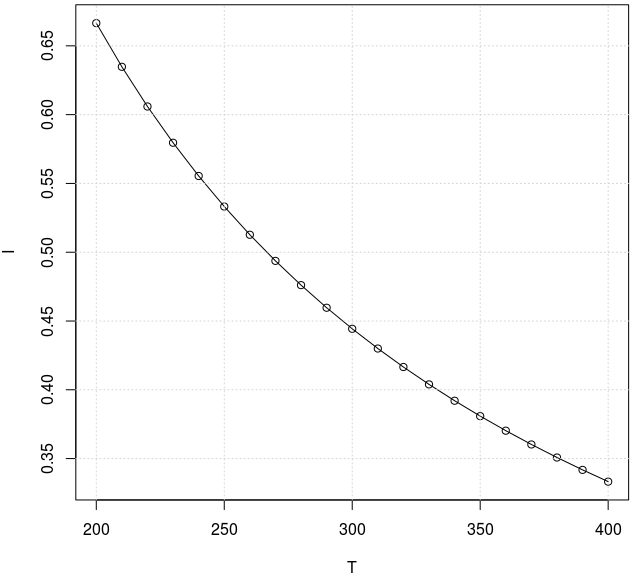
\includegraphics[width=12.5cm, height=12.5cm]{lat.png}

Рисунок 7.1 --- закон изменения значений функционала качества при разных временных отрезках. 
\end{center}

Из рисунка $7.1$ можно делать вывод, что при увеличении времени $T$ количество энергии $I$, которое требуется затратить на управление, уменьшается.
Это легко объясняется тем, что при увелечении затрат энергии на управление увеличивается угловая скорость, и следовательно меньше времени 
затрачивается на поворот.


\section{Разные весовые множители функционала качества}

Рассмотрим теперь случаи при одинаковом параметре $T\ =\ 300c$ и разных значениях весовых множителей $\alpha_1,\ \alpha_2,\ \alpha_3.$
Начальное положение тела также задано углами $(7.1)$.

\begin{itemize}
\item[1)]  Зафиксируем значения двух весовых множителей и будем варьировать значением третьего множителя.
Пусть $\alpha_1\ =\ 1000,\ \alpha_2\ =\ 2000$, $\alpha_3$ пробегает по значениям: 1000, 2000, ... 10000.

\begin{center}
   \begin{tabular}{ |l|l|l|l| }
   \multicolumn{4}{c}{Таблица 7.2}\\
    \hline
    \multicolumn{1}{|c|}{$\alpha_1$} & \multicolumn{1}{c|}{$\alpha_2$} & \multicolumn{1}{c|}{$\alpha_3$} & \multicolumn{1}{c|}{$I$} \\ \hline
    1000 & 2000 & 1000 & 0.2561562129231243  \\ \hline
    1000 & 2000 & 2000 & 0.3504523223918996  \\ \hline
    1000 & 2000 & 3000 & 0.44435544985946895  \\ \hline
    1000 & 2000 & 4000 & 0.5378731541347116  \\ \hline
    1000 & 2000 & 5000 & 0.631005289929338  \\ \hline
    1000 & 2000 & 6000 & 0.7237495719395564  \\ \hline
    1000 & 2000 & 7000 & 0.8161023547512606  \\ \hline
    1000 & 2000 & 8000 & 0.9080588213038621  \\ \hline
    1000 & 2000 & 9000 & 0.9996130262325005  \\ \hline
    1000 & 2000 & 10000 & 1.0907578924280608  \\ \hline
  \end{tabular}             
\end{center}

\begin{center}
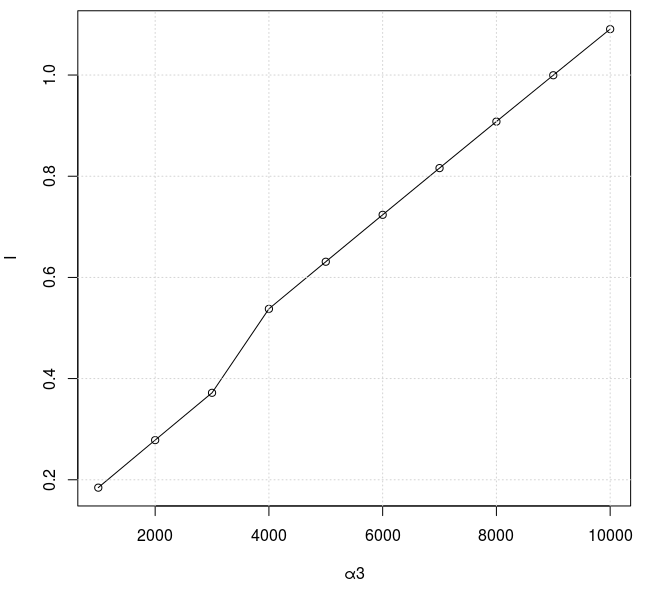
\includegraphics[width=10cm, height=10cm]{laa1.png}

Рисунок 7.2 --- закон изменения значений функционала качества при $\alpha_1\ =\ 1000,\ \alpha_2\ =\ 2000$. 
\end{center}

Из графика на рисунке $7.2$ видно, что между изменяемым параметром $\alpha_3$ и значением величины функционала качества $I$
существует линейная зависимость.


\item[2)] Теперь зафиксируем значение одного весового множителя и будем варьировать одинаковым образом значения двух остальных множителей:

\begin{center}
   \begin{tabular}{ |l|l|l|l| }
   \multicolumn{4}{c}{Таблица 7.3}\\
    \hline
    \multicolumn{1}{|c|}{$\alpha_1$} & \multicolumn{1}{c|}{$\alpha_2$} & \multicolumn{1}{c|}{$\alpha_3$} & \multicolumn{1}{c|}{$I$} \\ \hline
    1000 & 1000 & 1000 & 0.18455058244466496   \\ \hline
    1000 & 2000 & 2000 & 0.3504523223918996  \\ \hline
    1000 & 3000 & 3000 & 0.5163281860856808  \\ \hline
    1000 & 4000 & 4000 & 0.6821975645883387  \\ \hline
    1000 & 5000 & 5000 & 0.8480643431827684  \\ \hline
    1000 & 6000 & 6000 & 1.0139298219178696  \\ \hline
    1000 & 7000 & 7000 & 1.1797945575930033  \\ \hline
    1000 & 8000 & 8000 & 1.3456588291157578  \\ \hline
    1000 & 9000 & 9000 & 1.5115227892739374  \\ \hline
    1000 & 10000 & 10000 &  1.6773865337492355 \\ \hline
  \end{tabular}             
\end{center}

\begin{center}
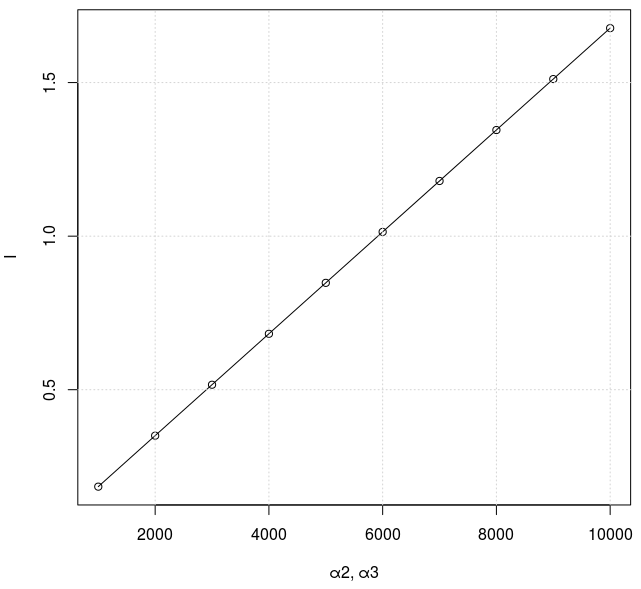
\includegraphics[width=10cm, height=10cm]{laa2.png}

Рисунок 7.3 --- закон изменения значений функционала качества при $\alpha_1\ =\ 1000$. 
\end{center}

Как и в первом случае, здесь линейная зависимость между изменяемыми параметрами $\alpha_1, \alpha_2$ и $I$.

\item[3)] Рассмотрим, наконец, случай, в котором все весовые множители варьируются одинаковым образом  

\begin{center}
   \begin{tabular}{ |l|l|l|l| }
   \multicolumn{4}{c}{Таблица 7.4}\\
    \hline
    \multicolumn{1}{|c|}{$\alpha_1$} & \multicolumn{1}{c|}{$\alpha_2$} & \multicolumn{1}{c|}{$\alpha_3$} & \multicolumn{1}{c|}{$I$} \\ \hline
    1000 & 1000 & 1000 & 0.18455058244466496   \\ \hline
    2000 & 2000 & 2000 & 0.3691011649278124  \\ \hline
    3000 & 3000 & 3000 & 0.5536517473623023  \\ \hline
    4000 & 4000 & 4000 & 0.7382023299085259  \\ \hline
    5000 & 5000 & 5000 & 0.9227529126527748  \\ \hline
    6000 & 6000 & 6000 & 1.1073034950203156  \\ \hline
    7000 & 7000 & 7000 & 1.2918540774575527  \\ \hline
    8000 & 8000 & 8000 & 1.4764046594125089  \\ \hline
    9000 & 9000 & 9000 & 1.660955240413333 \\ \hline
    10000 & 10000 & 10000 &  1.8455058248796425 \\ \hline
  \end{tabular}             
\end{center}

\begin{center}
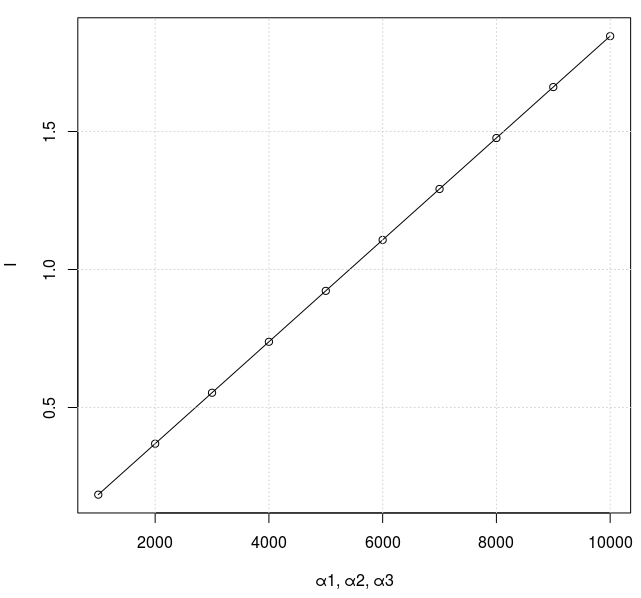
\includegraphics[width=10cm, height=10cm]{laa3.png}

Рисунок 7.4 --- закон изменения значений функционала качества при разных значениях весовых множителей. 
\end{center}

\end{itemize}

Таким образом, можно сделать вывод из графиков $7.2 - 7.4$, что при увелечении весовых множителей функционала качества
энергетические затраты на поворот тела растут, причем зависимость этого роста линейная.

\section{Разные начальные углы поворота}

В двух первых случаях рассматривалась зависимость значений функционала качества и его параметров при некотором фиксированном начальном положении тела.
Рассмотрим теперь значения функционала качества при разных начальных положениях твердого тела. Для этого зафиксируем конечное положение тела, которое 
задано углами Эйлера: $\widetilde\alpha\ =\ 0^{\circ},\ \widetilde\beta\ =\ 0^{\circ},\ \widetilde\gamma\ =\ 0^{\circ}$, весовые множители 
$\alpha_i, i\ =\ \overline{1, 3}$, где $\alpha_1 = 1000,\ \alpha_2 = 2000,\ \alpha_3 = 3000$ и время $T\ =\ 300c$. Начальное положение тела будем менять
в соответствии с таблицей 7.5. В этой же таблице даны соответствующие значения функционала качества.

\begin{center}
   \begin{tabular}{ |l|l|l|l| }
   \multicolumn{4}{c}{Таблица 7.5}\\
    \hline
    \multicolumn{1}{|c|}{$\alpha$} & \multicolumn{1}{c|}{$\beta$} & \multicolumn{1}{c|}{$\gamma$} & \multicolumn{1}{c|}{$I$} \\ \hline
    $0^{\circ}$ & 0$^{\circ}$  & 0$^{\circ}$  &0.0    \\ \hline
    1$^{\circ}$ & 1$^{\circ}$  & 1$^{\circ}$  &0.006056692698154153    \\ \hline
    2$^{\circ}$  & 2$^{\circ}$  & 2$^{\circ}$  &0.02408215835432236    \\ \hline
    3$^{\circ}$  & 3$^{\circ}$  & 3$^{\circ}$  &0.05385534350818591    \\ \hline
    4$^{\circ}$  & 4$^{\circ}$  & 4$^{\circ}$  &0.09514985533820493    \\ \hline
    5$^{\circ}$  & 5$^{\circ}$  & 5$^{\circ}$  &0.1477341814913685    \\ \hline
    6$^{\circ}$  & 6$^{\circ}$  & 6$^{\circ}$  & 0.21137190897814612   \\ \hline
    7$^{\circ}$  & 7$^{\circ}$  & 7$^{\circ}$  & 0.28582194497504043   \\ \hline
    8$^{\circ}$  & 8$^{\circ}$  & 8$^{\circ}$  &0.3708387365805886    \\ \hline
    9$^{\circ}$  & 9$^{\circ}$  & 9$^{\circ}$  & 0.46617248981673004   \\ \hline
    10$^{\circ}$  & 10$^{\circ}$  & 10$^{\circ}$  &0.5715693910515096    \\ \hline
    11$^{\circ}$  & 11$^{\circ}$  & 11$^{\circ}$  &0.6867718203349862    \\ \hline
    12$^{\circ}$  & 12$^{\circ}$  & 12$^{\circ}$  &0.8115185700197344    \\ \hline
    13$^{\circ}$  & 13$^{\circ}$  & 13$^{\circ}$  &0.9455450560043213    \\ \hline
    \end{tabular}             
\end{center}

\begin{center}
   \begin{tabular}{ |l|l|l|l| }
   \hline
    \multicolumn{4}{|c|}{продолжение таблицы 7.5}\\ \hline
    \multicolumn{1}{|c|}{$\alpha$} & \multicolumn{1}{c|}{$\beta$} & \multicolumn{1}{c|}{$\gamma$} & \multicolumn{1}{c|}{$I$} \\ \hline
    14$^{\circ}$  & 14$^{\circ}$  & 14$^{\circ}$  &1.0885835236291768    \\ \hline
    15$^{\circ}$  & 15$^{\circ}$  & 15$^{\circ}$  &1.2403632727704637    \\ \hline
    16$^{\circ}$  & 16$^{\circ}$  & 16$^{\circ}$  &1.4006108189429844    \\ \hline
    17$^{\circ}$  & 17$^{\circ}$  & 17$^{\circ}$  &1.5690501304510134    \\ \hline
    18$^{\circ}$  & 18$^{\circ}$  & 18$^{\circ}$  &1.7454027952571545    \\ \hline
    19$^{\circ}$  & 19$^{\circ}$  & 19$^{\circ}$  &1.929388211767391    \\ \hline
    20$^{\circ}$  & 20$^{\circ}$  & 20$^{\circ}$  &2.1207237623553117    \\ \hline
    21$^{\circ}$  & 21$^{\circ}$  & 21$^{\circ}$  &2.319124980674097    \\ \hline
    22$^{\circ}$  & 22$^{\circ}$  & 22$^{\circ}$  &2.5243057234840194    \\ \hline
    23$^{\circ}$  & 23$^{\circ}$  & 23$^{\circ}$  &2.735978298083406    \\ \hline
    24$^{\circ}$  & 24$^{\circ}$  & 24$^{\circ}$  &2.9538536340429173    \\ \hline
    25$^{\circ}$  & 25$^{\circ}$  & 25$^{\circ}$  &3.1776413757372017    \\ \hline
    26$^{\circ}$  & 26$^{\circ}$  & 26$^{\circ}$  &3.4070500639069183    \\ \hline
    27$^{\circ}$  & 27$^{\circ}$  & 27$^{\circ}$  &3.641787193331258    \\ \hline
    \end{tabular}             
\end{center}

\begin{center}
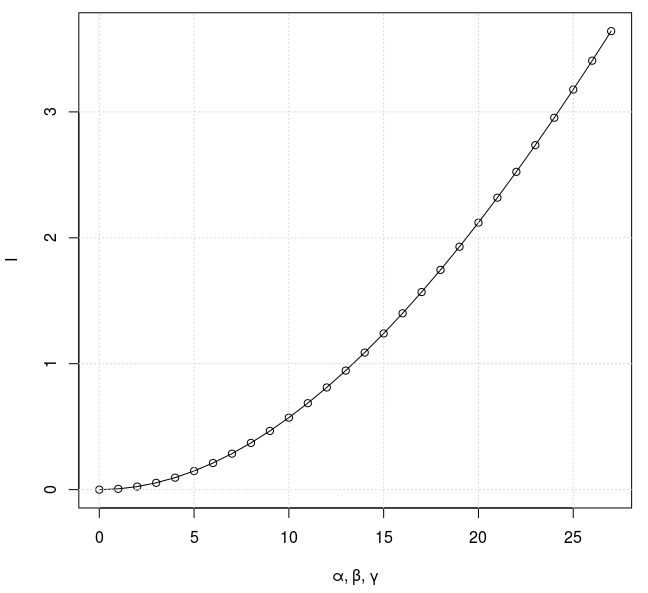
\includegraphics[width=10cm, height=10cm]{va.png}

Рисунок 7.5 --- закон изменения значений функционала качества при разных начальных углов поворота. 
\end{center}

График на рисунке $7.5$ показывает очевидную закономерность --- чем больше начальное отклонение тела от конечного его положения,
тем больше требуется энергетических затрат на управление.

Таким образом, в пунктах $7.1\ -\ 7.3$ были рассмотрены основные закономерности поставленной задачи оптимального управления $(4.1) - (4.4)$
для функционала качества $(4.5)$ при различных параметрах задачи путем анализа решения соответствующей краевой задачи $(5.12)$. Несмотря на то, что характер большинства этих зависимостей
можно определить из вида самого функционала качества, это позволяет лишний раз убедиться в эффективности выбранных методов для решения задачи,
а также корректности программной реализации. 

\newpage
\chapter{Примеры для больших углов поворота}

Расмотрим задачу оптимального управления, которой соответствует краевая задача $(8.1)$ для тела, начальное положение которого задано углами Эйлера:
$\alpha\ =\ -78.4^{\circ},\ \beta\ =\ -39.9^{\circ},\ \gamma\ =\ 112.9^{\circ}$,
а конечное --- $\widetilde\alpha\ =\ 0^{\circ},\ \widetilde\beta\ =\ 0^{\circ},\ \widetilde\gamma\ =\ 0^{\circ}$. 
Пусть требуется решить задачу с точностью $\varepsilon = 10^{-9}$ при весовых множителях $\alpha_1 = 1000,\ \alpha_2 = 2000,\ \alpha_3 = 3000$ для времени
$T\ =\ 300 c$.

\begin{equation}
\begin{cases}
2\boldsymbol{\dot{\Lambda}}\ =\ \boldsymbol{\Lambda} \circ \boldsymbol\Omega,\\
 \boldsymbol\Lambda(0)\ =\ \boldsymbol{\Lambda^{0}}(\lambda_0^{0},\ (\lambda_1^{0},\ \lambda_2^{0},\ \lambda_3^{0})), \\
 \lambda_{0}^{0}\ =\ -0.5821271946729387, \\
 \lambda_{1}^{0}\ =\ 0.10821947847990215, \\
 \lambda_{2}^{0}\ =\ 0.641192910029563, \\
 \lambda_{3}^{0}\ =\-0.48814764756943485. \\
 \boldsymbol\Lambda(T)\ =\ \boldsymbol{\Lambda^{T}}(\lambda_0^{T},\ (\lambda_1^{T},\ \lambda_2^{T},\ \lambda_3^{T})), \\
 \lambda_{0}^{T}\ =\ 1, \ 
 \lambda_{1}^{T}\ =\ 0, \ 
 \lambda_{2}^{T}\ =\ 0, \ 
 \lambda_{3}^{T}\ =\ 0. \ 
 \end{cases}
\end{equation}

График изменения компонент кватерниона $\boldsymbol\Lambda\ =\ \boldsymbol\Lambda(\lambda_0,\ (\lambda_1,\ \lambda_2, \lambda_3))$ с течением времени,
найденный в ходе решения, представлен на рисунке $8.1$. По данному рисунку видно, что оптимальное управление переводит тело из заданного начального
углового положения в требуемое конечное.

Найденное решение $\boldsymbol\Lambda(t)$ позволяет получить данные об изменениях углов Эйлера, задающие угловое положение тела.
На рисунках $8.2\ -\ 8.4$ представлены изменения углов прецессии, нутации, собственного вращения соответственно.

\begin{center}
\vspace*{50px}
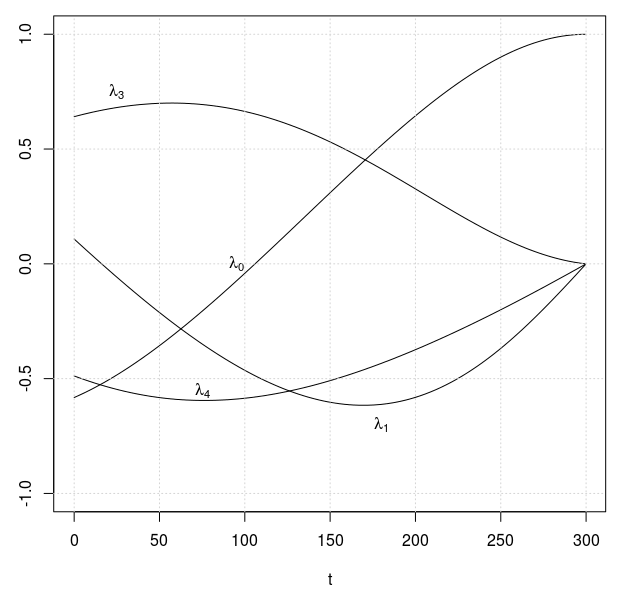
\includegraphics[width=17cm, height=17cm]{l300.png}

Рисунок $8.1$ --- график изменения компонент оптимальной траектории. 
\end{center}

\begin{center}
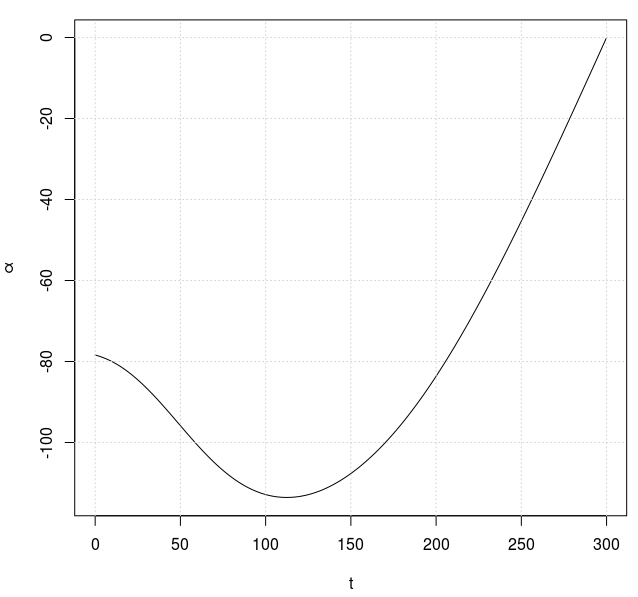
\includegraphics[width=11cm, height=11cm]{alpha.png}

Рисунок $8.2$  --- изменение угла прецессии. 
\end{center}

\begin{center}
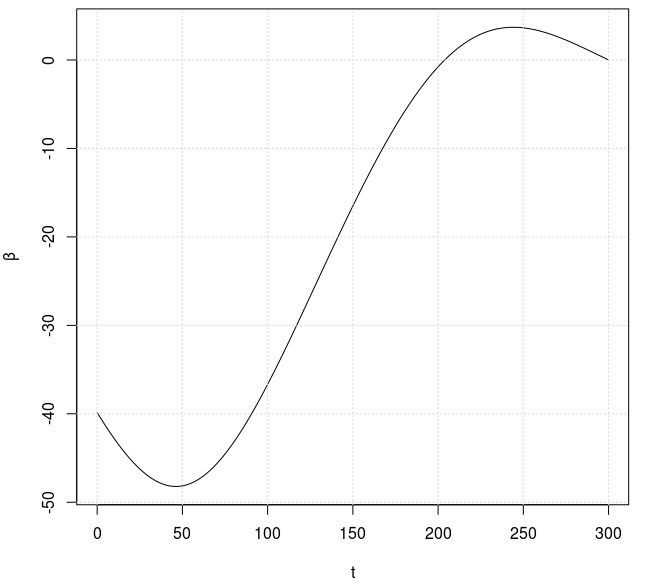
\includegraphics[width=11cm, height=11cm]{beta.png}

Рисунок $8.3$  --- изменение угла нутации. 
\end{center}

\begin{center}
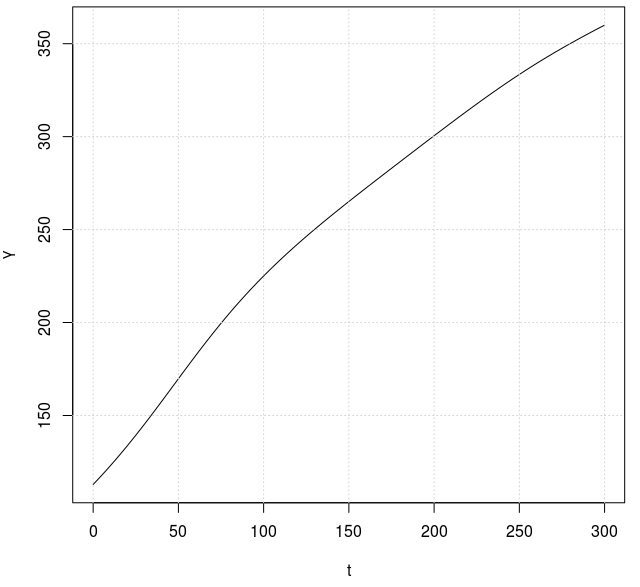
\includegraphics[width=11cm, height=11cm]{gamma.png}

Рисунок $8.4$  --- изменение угла собственного вращения. 
\end{center}

Рисунки $8.2\ -\ 8.4$ полностью соответствуют рисунку $8.1$, и следовательно требованиям для оптимального управления.

В поставленной задаче в качестве оптимального управления, как было сказано ранее, выступает угловая скорость
$\boldsymbol\Omega = \boldsymbol\Omega(\omega_0,\ (\omega_1,\ \omega_2,\ \omega_3))$, которая также находится в ходе решения краевой задачи $(5.12)$. График изменения
компонент угловой скорости $\omega_1,\ \omega_2,\ \omega_3$ представлен на рисунке $8.5$.

Основная трудность, с которой можно столкнуться при решении задачи оптмального управления для больших углов отклонения между начальным и конечным
положениями тела --- это нахождение начального приближения $\Psi$, поэтому желательно знать, где приблизительно его нужно искать. 

Для данной задачи график изменения компонент кватерниона $\boldsymbol\Psi\ =\ \boldsymbol\Psi(\psi_0,\ (\psi_1,\ \psi_2, \psi_3))$, который получается на последней итерации
метода Ньютона решения краевой задачи $(5.12)$, представлены на рисунке $8.6$.

\begin{center}
\vspace*{50px}
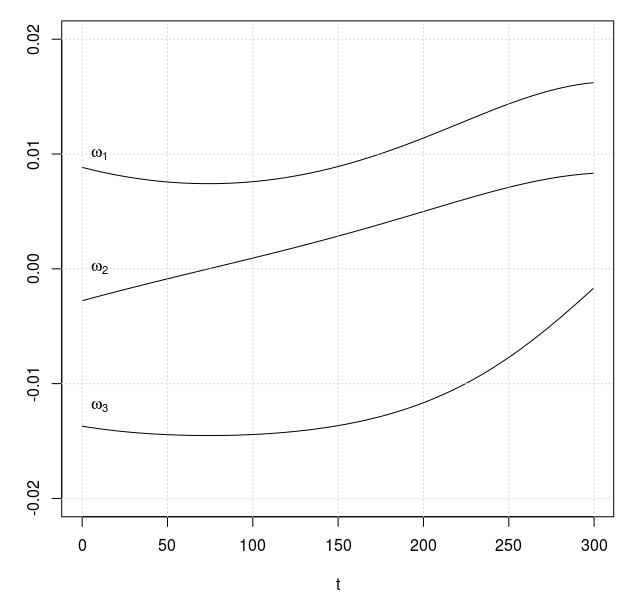
\includegraphics[width=17cm, height=17cm]{o300.png}

Рисунок $8.5$ --- график изменения компонент оптимального управления.
\end{center}


\begin{center}
\vspace*{50px}
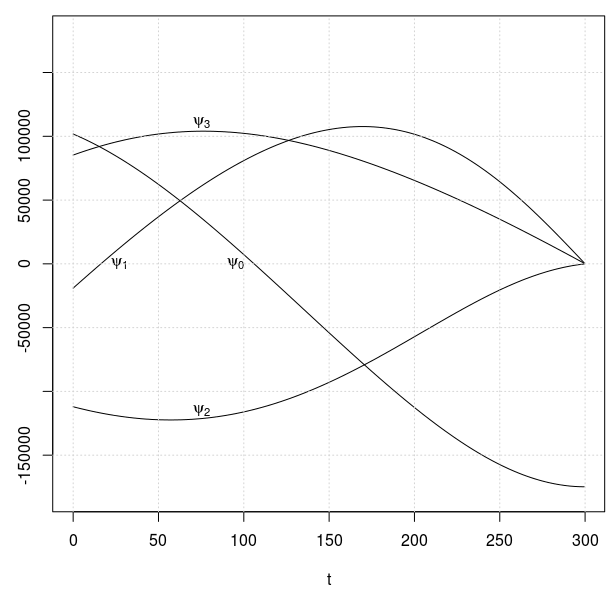
\includegraphics[width=17cm, height=17cm]{p300.png}

Рисунок $8.6$ --- график изменения компонент кватерниона $\Psi$.
\end{center}

Рассмотрим теперь задачу $(8.1)$ при $T\ =\ 301c,\ и\ T\ =\ 302c$. Значения функционала качества при таких параметрах $T$, включая случай $T\ =\ 300c$
представлены в таблице $8.1$.

\begin{center}
   \begin{tabular}{ |l|l|l|l| }
   \multicolumn{2}{c}{Таблица 8.1}\\
    \hline
    \multicolumn{1}{|c|}{$T$, c} & \multicolumn{1}{c|}{$I$} \\ \hline
    300  & 143.0483289121585   \\ \hline
    301  & 142.5730831794837  \\ \hline
    302  & 142.10098482727184\\ \hline
    \end{tabular}             
\end{center}

Графическое представление таблицы $8.1$ отражено на рисунке $8.7$, из которого следует, что при увелечении параметра $T$ энергетические затраты
на управление уменьшаются, что соответствует выводам, сделанных для малых углов отклонения.

\begin{center}
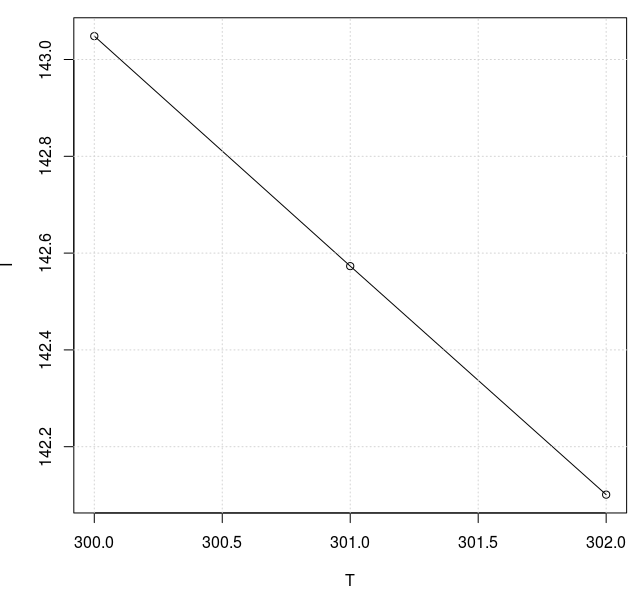
\includegraphics[width=10cm, height=10cm]{ba.png}

Рисунок 8.7 --- графическое представление таблицы $8.1$. 
\end{center}

\newpage

\conclusions

В предоставленной квалификационной работе удалось решить задачу оптимального управления углового движения ИСЗ, 
для которой требовалось составить и решить краевую задачу с помошью принципа максимума Л.С. Понтрягина. 

Были рассмотрены различные поведения системы при различных параметрах. Также удалось программно реализовать алгоритм численного решения задачи
с применением алгебры кватернионов.

Полученные в работе теоретические результаты позволяют понять основные зависимости функционала качества управления и его параметров,
а также прогнозировать поведение системы при изменениях параметров самой задачи.

\begin{thebibliography}{9}
\bibitem{Chelnokov:2006:Kvat_Bikvat} 
Челноков, Ю. Н.
\textit{Кватернионные и бикватернионные модели и методы механики твёрдого тела и их приложения}. 
М.: Физматлит, 2006. – 512c.
 
\bibitem{Branetz_Shmyglevsky:1973:Prim_Kvat_orient} 
Бранец, В. Н., and Шмыглевский, И. П.
\textit{Применение кватернионов в задачах ориентации твердого тела}. 
М.: Наука, 1973. – 320c.

\bibitem{Pontryagin:1983:Matem_theory} 
Понтрягин, Л. С., and Болтянский, В. Г. and Гамкрелидзе, Р. В. and  Мищенко, Е. Ф.
\textit{Математическая теория оптимальных процессов}. 
М.: Наука, 1983 – 393c.

\bibitem{Sapunkov:2001:Chisl_issl_SAU} 
Сапунков, Я. Г.
\textit{Численное исследование систем автоматического управления}. 
М.: Наука, 2001. – 24c.	
	
\bibitem{Gorelov} 
Горелов Ю.Н.
\textit{Численные методы решения обыкновенных дифференциальных уравнений (Метод Рунге - Кутта)}. 
Изд-во «Самарский университет», 2006. – 48 с.		

\bibitem{A.S.Antipova, V.G.Birukov} 
Антипова А.С., Бирюков Б.Г.
\textit{Аналитическое и численное исследование  кинематической задачи оптимальной переориентации твердого тела}. 
УДК – 48 с.	

\bibitem{V.S. Aslanov} 
Асланов. В. С.
\textit{Динамика твёрдого тела и систем тел}. 
Самарский государственный аэрокосмический университет, 2011  – 216с.

\bibitem{Tarasov} 
Тарасов В.Н., Бахарева Н.Ф. 
\textit{Численные методы. Теория, алгоритмы, программы.}. 
Оренбург: ИПК ОГУ, 2008. – 264 с. 

\bibitem{Ermolin} 
Ермолин В. С., Королев В. С., Потоцкая Е. Ю.
\textit{Теоретическая механика. Часть I. Кинематика. Учебное пособие.}. 
СПб: СПбГУ, ВВМ, 2013.— 225 с. 

\bibitem{Telyakovskiy} 
Теляковский С. А.
\textit{Курс лекций по математическому анализу}. 
М.: МИАН, 2009. – 212 с.

\bibitem{Panteleev} 
Пантелеев А.В., Бортаковский А.С., Летова Т.А.
\textit{Оптимальное управление в примерах и задачах.}. 
М: Издательство МАИ, 1996. — 583 с. 

\bibitem{knuthwebsite} 
Knuth: Computers and Typesetting,
\\\texttt{\small{http://www-cs-faculty.stanford.edu/\~{}uno/abcde.html}}
(дата последнего обращения: 10.05.16)

\bibitem{Page11gauss.pdf} 
Прямые методы решения линейных систем
\\\texttt{\small{http://www.math.spbu.ru/user/pan/Page11-gauss.pdf}}
(дата последнего обращения: 10.05.16)

\bibitem{info00036.htm} 
Метод Гаусса
\\\texttt{\small{http://pedsovet.info/info/pages/referats/info\_00036.htm}}
(дата последнего обращения: 10.05.16)

\bibitem{Euler_angles} 
Углы Эйлера
\\\texttt{\footnotesize {https://ru.wikipedia.org/wiki/\%D0\%A3\%D0\%B3\%D0\%BB\%D1\%8B\_\%D0\%AD\%D0\%B9\%D0\%BB\%D0\%B5\%D1\%80\%D0\%B0}}
(дата последнего обращения: 10.05.16)

\bibitem{Conversion_between_quaternions_and_Euler_angles} 
Conversion between quaternions and Euler angles
\\\texttt{\small{http://en.wikipedia.org/wiki/Conversion\_between\_quaternions\_and\_Euler\_angles}}
(дата последнего обращения: 10.05.16)

\bibitem{Newton's method} 
Newton's method
\\\texttt{\small{https://en.wikipedia.org/wiki/Newton\%27s\_method}}
(дата последнего обращения: 10.05.16)

\bibitem{Newton's method} 
Java Platform, Standard Edition (Java SE) 8
\\\texttt{\small{https://docs.oracle.com/javase/8/}}
(дата последнего обращения: 10.05.16)

\bibitem{What Is an Interface?} 
Java: What Is an Interface?
\\\texttt{\small{https://docs.oracle.com/javase/tutorial/java/concepts/interface.html}}
(дата последнего обращения: 10.05.16)

\bibitem{What Is an Interface?} 
R: Documentation
\\\texttt{\small{https://www.r-project.org/other-docs.html}}
(дата последнего обращения: 10.05.16)

\bibitem{What Is an Interface?} 
Block diagram
\\\texttt{\small{https://en.wikipedia.org/wiki/Block\_diagram}}
(дата последнего обращения: 10.05.16)

\end{thebibliography}

\Appendix % Приложения

\chapter{Структура программы}

\begin{center}
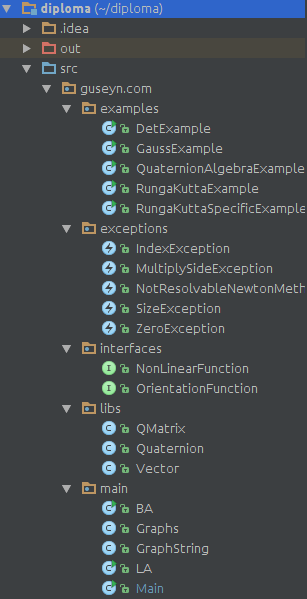
\includegraphics[width=10cm, height=20cm]{s1.png}

\end{center}

\begin{center}
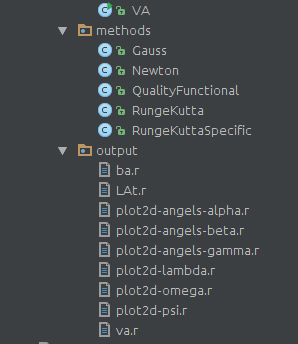
\includegraphics[width=10cm, height=12cm]{s2.png}

\end{center}

\chapter{Исходный код программы \label{AppendixB}}

\lstset{ %
language=Java,                 % выбор языка для подсветки 
basicstyle=\small\sffamily, % размер и начертание шрифта для подсветки кода
numbers=left,               % где поставить нумерацию строк (слева\справа)
numberstyle=\tiny,           % размер шрифта для номеров строк
stepnumber=1,                   % размер шага между двумя номерами строк
numbersep=5pt,                % как далеко отстоят номера строк от подсвечиваемого кода
backgroundcolor=\color{white}, % цвет фона подсветки - используем \usepackage{color}
showspaces=false,            % показывать или нет пробелы специальными отступами
showstringspaces=false,      % показывать или нет пробелы в строках
showtabs=false,             % показывать или нет табуляцию в строках
frame=single,              % рисовать рамку вокруг кода
tabsize=2,                 % размер табуляции по умолчанию равен 2 пробелам
captionpos=t,              % позиция заголовка вверху [t] или внизу [b] 
breaklines=true,           % автоматически переносить строки (да\нет)
breakatwhitespace=false, % переносить строки только если есть пробел
escapeinside={\%*}{*)}   % если нужно добавить комментарии в коде
}

\lstinputlisting[language=Java, caption=Quaternion.java]{com/libs/Quaternion.java}
\lstinputlisting[language=Java, caption=Vector.java]{com/libs/Vector.java}
\lstinputlisting[language=Java, caption=QMatrix.java]{com/libs/QMatrix.java}

\lstinputlisting[language=Java, caption=NonLinearFunction.java]{com/interfaces/NonLinearFunction.java}
\lstinputlisting[language=Java, caption=OrientationFunction.java]{com/interfaces/OrientationFunction.java}

\lstinputlisting[language=Java, caption=IndexException.java]{com/exceptions/IndexException.java}
\lstinputlisting[language=Java, caption=MultiplySideException.java]{com/exceptions/MultiplySideException.java}
\lstinputlisting[language=Java, caption=NotResolvableNewtonMethodException.java]{com/exceptions/NotResolvableNewtonMethodException.java}
\lstinputlisting[language=Java, caption=SizeException.java]{com/exceptions/SizeException.java}
\lstinputlisting[language=Java, caption=ZeroException.java]{com/exceptions/ZeroException.java}

\lstinputlisting[language=Java, caption=Gauss.java]{com/methods/Gauss.java}
\lstinputlisting[language=Java, caption=Gauss.java]{com/methods/Newton.java}
\lstinputlisting[language=Java, caption=QualityFunctional.java]{com/methods/QualityFunctional.java}
\lstinputlisting[language=Java, caption=RungeKutta.java]{com/methods/RungeKutta.java}
\lstinputlisting[language=Java, caption=RungeKuttaSpecific.java]{com/methods/RungeKuttaSpecific.java}

\lstinputlisting[language=Java, caption=Main.java]{com/main/Main.java}

\end{document}
